
\documentclass[11pt,twoside,a4paper]{article}
\usepackage[hmargin=2cm, vmargin=2cm]{geometry}
\usepackage{microtype}
\usepackage{graphicx}
\usepackage{hyperref}
\usepackage[english]{babel}
\usepackage{setspace}
\usepackage{xcolor}
\usepackage{multicol}
\usepackage{float}
\usepackage{amsmath}
\usepackage{amsthm}
\usepackage{amssymb}
\usepackage{hyperref}
\usepackage[font=small,skip=2pt]{caption}
\usepackage[
backend=biber,
style=authoryear-comp,
]{biblatex}


\newcommand{\independent}{\perp\!\!\!\!\perp} 

\addbibresource{RMbibliography.bib}
\onehalfspacing
\parindent=0pt

\begin{document}
	\title{{\LARGE Model Selection for Scalar-on-Function Regression \\ with Applications to Near-Infrared Spectroscopy}}
	\author{Jonghun Baek, Jakob R. Juergens, Jonathan Willnow}
	\date{11.02.2022}
	\maketitle
	\vspace{1.5 cm}
	\begin{center}
		Research Module in Econometrics and Statistics \\
		Winter Semester 2021/2022
	\end{center}
	
	\newpage
	
	\tableofcontents
	
	\newpage
	
	\section{Colour Guide}
		\begin{itemize}
			\item {\color{red} RED}: is for general comments for your own text
			\item {\color{green} GREEN}: is for Jona's comments
			\item {\color{orange} ORANGE}: is for Jonghun's comments
			\item {\color{blue} BLUE}: is for Jakob's comments
		\end{itemize}
	
	\section{Introduction}
	
	\begin{itemize}
		\item Describe the idea of regressing a scalar on functional data
		\item Describing the difference to multiple linear regression intuitively
		\item Giving an intuitive example
	\end{itemize}	
	Functional Data Analysis (FDA) is {\color{red} (roots in the 1940s Grenander and Karhunen)} gaining more attention as researchers from different fields collect data that is functional in nature. Although classical statistical methods can often process this data, but only FDA allows extracting the information given by the smoothness of the underlying process of the functional data (cf. \cite{levitin_introduction_2007}).
	 As \cite{kokoszka_introduction_2017} describe, FDA should be considered when one can view variables or units of a given data set as smooth curves or functions and the interest is in analyzing samples of curves (cf. \cite[S.~17]{kokoszka_introduction_2017}).\\
	 
		
			 This measurement set can be viewed as set of discretized approximations of the underlying true process which could be the absorption of the Near-infrared (NIR) spectrum which will be used for the simulation and application. NIR-spectroscopy uses the near-infrared region of the electromagnetic spectrum (780nm to 2500nm) to measure the absorption of its waves on a sample to analyse the interaction of each other. {\color{green} For more details refer to the appendix SECTION ??!??!}. This continuous underlying process for which 
 $x_i(t)$ exists $\forall t \in [T_1, T_2]$ is only observed at the discrete measurement points. This dataset can then be used to perform Functional Linear Regression (FLR) on a scalar response variable. To conduct functional linear regression, several new concepts and methods need to be considered and explained that distinguish it multivariate linear regression.
%	 In economics, one application could be the regression of stock market correlations on the Global Crisis Index (GCI) to where the regression allows to assess the relationship between the correlation and the GCI at every point within a window (cf. \cite{Das_2019}).\\
The focus of this paper is to introduce FLR in a scalar-on-function setting. We will be using the standard FLR framework, which relates functional predictors to a scalar response as follows:
	 
	 \begin{equation}
	 	Y(\omega) = \alpha + \int_{0}^{1}{X(\omega)(s)\beta(s) \mathrm{d}s} + \epsilon(\omega),
	 	\qquad i = 1, ..., n
	 \end{equation}
 
	 where the $X_{i}$ are realizations of a random function $\mathbf{X}$, $Y_i$ are the corresponding realizations of the response variable and $\beta(s)$ is the coefficient function. The distinct feature of this framework is that the regressor is a function, which necessitates a different approach to estimation. As in the well-known framework of scalar linear regression, this is motivated by an interest in $\beta(s)$ for prediction. For instance, fluctuation in $X_i(s)$ at a point $s_0$ will not have any effect on $Y_i$ if $\beta(s_0)$ = 0. \\
	 Estimation of $\beta(s)$ is inherently an infinite-dimensional problem. In Section 2, after introducing the necessary theoretical concepts, we describe three methods of estimating a scalar coefficient function using a concept called truncated basis expansion. We report the results of the Monte-Carlo simulation regarding these three different methods in Section 3. Finally, in Section 4, we test the prediction of FLR in a real-world setting. {\color{red} (We may put some simple descriptions of results about each of MC and Application)}

	\section{Theory}
	In multivariate regression, data is often observed in the form of elements from Euclidean space, $\mathbb{R}^p$. However, the statistics derived from infinite-dimensional random functions cannot be defined on a finite dimensional space. To understand functional linear regression and the differences between the methods presented in this paper, it is therefore necessary to introduce some concepts and extend known aspects of linear regression theory to include functional objects. One integral concept in inferential statistics are random variables. Paraphrasing a definition by \cite{bauer_wahrscheinlichkeitstheorie_2020}, a random variable $X:\Omega \rightarrow \Omega'$ is an $\mathcal{A} \text{-} \mathcal{A'} \text{-measurable}$ function, where $(\Omega, \mathcal{A}, P)$ is a probability space and $(\Omega', \mathcal{A'})$ is a measure space.\\
	A typical case known to every undergraduate student of economics in less formal detail is $(\Omega', \mathcal{A'}) = (\mathbb{R}, \mathcal{B})$, where $\mathcal{B}$ is the canonical $\sigma$-algebra on the real numbers. As a first intuition, it is possible to imagine a similar concept where a random variable does not realize as an element of the real numbers but as a function in a function space. A formalization of this idea makes some more theoretical considerations necessary. The following theoretical introduction closely follows chapters 2.3 and 2.4 from \cite{hsing_theoretical_2015}. 
	
	\subsection{Inner Products and Hilbert Spaces}
	Let $\mathbb{V}$ be a vector space over some field of scalars $\mathbb{F}$. In the following we restrict our analysis to the case of $\mathbb{F} = \mathbb{R}$. A function $\langle \cdot, \cdot \rangle : \mathbb{V} \times  \mathbb{V} \rightarrow \mathbb{F}$ is called an inner product, if $\forall v, v_1, v_2 \in \mathbb{V}$ and $a_1, a_2 \in \mathbb{F}$ the following properties hold.
	
	\begin{multicols}{2}
		\begin{enumerate}
			\item $\langle v, v \rangle \geq 0$
			\item $\langle v, v \rangle = 0$ if $v = 0$
			\item $\langle a_1 v_1 + a_2 v_2, v \rangle = a_1 \langle v_1, v \rangle + a_2 \langle v_2, v \rangle$
			\item $\langle v_1, v_2 \rangle = \langle v_2, v_1 \rangle$
		\end{enumerate}
	\end{multicols}

	A vector space with an associated inner product is called an inner product space. {\color{red}[verbatim quote!]}
	The inner product naturally defines a norm and an associated distance on the vector space as follows.
	
	\begin{equation}
		\lvert \lvert v \rvert \rvert = {\langle v, v \rangle}^{\frac{1}{2}}
	\end{equation}

	\begin{equation}
		d(v_1, v_2) = {\langle v_2 - v_1, v_2 - v_1 \rangle}^{\frac{1}{2}}
	\end{equation}
	
	If the inner product space is complete with respect to the induced distance, it is called a Hilbert space, denoted $\mathbb{H}$ in the following. To extend the known concept of a basis in a finite dimensional space to the potentially infinite Hilbert spaces, it is necessary to define the closed span of a sequence of elements of $\mathbb{H}$. Recall that the span of a set of vectors $S \subseteq \mathbb{R}^P$ is given by
	
	\begin{equation}
		span(S) = \left\{\sum_{i = 1}^{k} \lambda_i v_i \: \bigg\vert \: k \in \mathbb{N}, \: v_i \in S, \: \lambda_i \in \mathbb{R} \right\}
	\end{equation}
			
	The closed span $\overline{span}(S)$ of a sequence $S$ in $\mathbb{H}$ is defined as the closure of the span with respect to the distance induced by the norm. $S$ is called a basis of $\mathbb{H}$ if $\overline{span}(S) = \mathbb{H}$. \\
	It is called an orthonormal basis, if in addition the following properties hold. 
	
	\begin{multicols}{2}
		\begin{enumerate}
			\item $\langle v_i, v_j \rangle = 0 \quad \forall v_i, v_j \in S \quad i \neq j$
			\item $\lvert \lvert v \rvert \rvert = 1 \quad \forall v \in S$
		\end{enumerate}
	\end{multicols}

	As in the case of a Banach space, each element of a Hilbert space can be expressed in terms of a corresponding basis. This can be done using a Fourier expansion of an element $x \in \mathbb{H}$ w.r.t. a basis $S = \{s_n\}$ as follows.
	
	\begin{equation}
		x = \sum_{j = 1}^{\infty}{\langle x, s_j \rangle}s_j
	\end{equation}
	
	As can be seen, differing from the case of a Banach space, these representations can be limits of series as previously hinted at by using the closed span of the basis. As using an infinite number of basis functions is infeasible in applied contexts, an intuitive way to approximate elements of a Hilbert space, is to use a truncated series.
	
	\begin{equation}
		x \approx \sum_{j = 1}^{K}{\langle x, s_j \rangle}s_j
	\end{equation}
	
	\subsection{Hilbert Space of Square-Integrable Functions{\color{orange} $\mathbb{L}^2[0,1]$ space and Random Function}}
	In functional data analysis, one Hilbert space of particular importance is the space of square-integrable functions on $[0,1]$ denoted $\mathbb{L}^2[0,1]$. To define it, look first at the measure space given by $([0,1], \mathcal{B}, \mu)$ where $\mathcal{B}$ is the Borel $\sigma$-algebra on $[0,1]$ and $\mu$ is the Lebesgue-measure. Then $\mathbb{L}^2[0,1]$ is the collection of all measurable functions $f$ on $[0,1]$ that fulfill the following condition.
	
	\begin{equation}
		\lvert \lvert f \rvert \rvert_2 = \int_{0}^{1} \lvert f \rvert^2 \mathrm{d}\mu < \infty
	\end{equation}
	
	All functions $f$ satisfying the above condition are called square-integrable functions. Moreover, it ensures that a random function has a finite second moment so that the variance and the covariance function can be defined. Its inner product is defined as
	
	\begin{equation}
		\langle f_1, f_2 \rangle = \int_{0}^{1} f_1 f_2 \mathrm{d}\mu.
	\end{equation}
	
	$\mathbb{L}^2[0,1]$ is the function space that is most often used for theoretical considerations in functional data analysis without loss of generality. We also focus on the interval [0,1] for the purpose of this paper.	A random function defined on $\mathbb{L}^2[0,1]$ can be represented as
	a function $X : \Omega \rightarrow \mathbb{L}^2[0,1]$ which is defined on a common probability space $(\Omega, \mathcal{A}, P)$ where $\Omega$ is a sample sapce with $\sigma$-algebra $\mathcal{A}$ and a probability space $P$. The realized $X(\omega)(t)$ for every $t \in [0,1]$ is called a sample curve for the process. The collection of such sample curves constitutes a functional data set.
	%Trivially, it is possible to extend this to other closed intervals on the reals line, but there are also more complex generalizations. For the purpose of this paper we will focus on the typical case and assume that random functions are random variables realizing in $\mathbb{L}^2$ for some closed interval of the real numbers. 
	
	%\begin{equation}
	%\{f(t,\omega) : t \in [0, 1], \omega \in \Omega\}
	%\end{equation}
	
	\subsection{Bases of $\mathbb{L}^2$ {\color{orange}Basis Representation for Functions}} 
	{\color{red} Maybe change title due to monomial and bspline basis not fulfilling this property.}
	As previously described, a basis of a Hilbert space can be used to express elements of the space using the corresponding Fourier expansion. Two examples of bases that are often used in practice to express / approximate elements of $\mathbb{L}^2[0,1]$  are explained in the following.
	
	Both of these can be used to express or in the case of the b-spline basis approximate elements of $\mathbb{L}^2[0,1]$ as a weighted sum of basis functions. Let therefore $\{\phi_i(t) \: \vert \: i \in \mathcal{I}\}$ be the basis used to express / approximate a realization $X(\omega_0) = x(t)$ of $X(\omega)$.
	
	\begin{equation}
		X(\omega_0) = x(t) = \sum_{j \in \mathcal{I}} A_{j}(\omega_0) \phi_j(t)
	\end{equation}
	
	\paragraph{Monomial Basis}
	{\color{red} No shift parameter in implementation in fda.} Every result of monomial basis expansion is the Taylor series of some function. 
	This is the basis that is needed to build polynomials, one of the best-known ways to expand a function. The polynomial of the form 

	\begin{equation}
		x(t) = \sum_{i \in \mathcal{I}} c_i(t -w)^{i}
	\end{equation}
	can be expressed as a finite linear combination of the monomials $(t - w)^{i}$ with coefficient $c_i$ which form the basis 
	
	\begin{equation}
		\phi_{i}^{M}(t) = (t-w)^k \quad i \in \mathcal{I}
	\end{equation}
	The single basis function $1$ within the monomial basis system, for $k=0$, is called the constant basis system (cf. \cite{horvath_inference_2012}). {\color{blue} Taylor expansion as motivation}\\ 
	The shift parameter $w$ usually is specified to be the center of the interval subject to approximation.
	 Problems of collinearity arise for higher degrees since the monomial basis becomes more correlated as the degrees increase. This restricts the number of degrees and therefore the use of this basis: For simple functions this may be useful, but the small number of degrees makes it impossible to capture pronounced local peculiarities and leads to undesirable behaviour at the tails. (cf. \cite{ramsay_functional_2005})


	
	\paragraph{Fourier Basis}
	The Fourier basis for $\mathbb{L}^2[0,1]$ is given by the following sequence of functions defined on $[0,1]$.
	\begin{equation}
		\phi_{i}^{F}(x) = 
		\begin{cases}
			1 & \text{if} \quad i = 1\\
			\sqrt{2} \cos(\pi i x) & \text{if} \quad i \quad \text{is even} \\
			\sqrt{2} \sin(\pi (i-1)x) & \text{otherwise}
		\end{cases}
	\end{equation}
	
	Therefore, its basis functions inherits a repeating behaviour which is useful to expand functions that represent an periodic or seasonal underlying process over the period $T$. Rephrasing from \cite{ramsay_functional_2005}, the Fourier basis functions are orthogonal when the values $t_j$ are equally spaced within $T$. This basis is suitable to expand functions with a similar curvature order across the domain, resulting generally in uniformly smooth expansions.  {\color{blue} Motivate from fourier series}

	\paragraph{B-spline Basis} Following chapter 3.5 from \cite{ramsay_functional_2005}, splines are defined by first dividing the interval of interest $[\tau_0, \tau_L]$ into $L$ subintervals of non-negative length divided by a non-decreasing sequence of points $(\tau_l)_{l = 1,\dots, L-1}$ called knots. On each subinterval, a spline is a polynomial of chosen order $m = n+1$ where $n$ is its degree. Additionally, at each $\tau_l$ the the polynomials on neighbouring subintervals must match derivatives up to order $m-2$.
	A B-spline is a spline belonging to a basis system developed by \cite{de_boor_practical_1978}. Let $\phi_{l,m}^{BS}(x) \quad l = 1,\dots,L-1$ be the B-spline of order $m$ for an interval $[\tau_0, \tau_L]$ and knots $\{\tau_l \: \vert \: l = 1,\dots, L-1\}$, then it is defined by the Cox-de Boor recursion formula as follows. 

	\begin{equation}
		\begin{split}
			\phi_{l,0}^{BS}(x) = &
			\begin{cases}
				1 & \text{if} \quad x \in \left[\tau_l, \tau_{l+1}\right)\\
				0 & \text{otherwise}
			\end{cases}\\ \\
			\phi_{l,m}^{BS}(x) = &\frac{x - \tau_l}{\tau_{l+m} - \tau_l} \phi_{l,m-1}^{BS}(x) + \frac{\tau_{l+m+1} - x}{\tau_{l+m+1} - \tau_{l+1}} \phi_{l+1,m-1}^{BS}(x)
		\end{split}
	\end{equation}
	
	This, however, does not really yield a basis of $\mathbb{L}^2[0,1]$ as the closed span of this finite sequence of functions is not equal to $\mathbb{L}^2[0,1]$. To really obtain a basis of $\mathbb{L}^2[0,1]$ from B-splines, further theoretical considerations about, for example, infinite series of B-splines and specific knot choices would have to be made. As this is out of the scope of this paper, for the sake of simplicity, we will assume that a B-spline basis representation of a function in $\mathbb{L}^2[0,1]$ will serve as a sufficient approximation for an appropriately chosen B-spline basis. 
	Even though, this approach is not theoretically exact, in practice, this is often a reasonable approach and yields satisfactory results in cases where the functional form of B-splines makes them an appropriate approximation tool. 
	
	{\color{red}Explain what happens when $l+m+1 > L$ !!!\\
		Additionally, modify for multiple knots at the boundaries to get better behavior at the boundaries. Needs some more explanation.}	
	
	\subsection{Approximation and Smoothing via Basis Truncation}
	As above-mentioned, the realized curves can be estimated with basis functions. For the basis expansion, it is technically possible to use all basis functions $b_{j \in \mathcal{I}}$. On the one hand, this way is not efficient since the technique with too many basis functions can even approximate a noise of the sample curves which possibly interrupts the analysis. On the other hand, the important information on the curves would be missed with a too-small number of basis functions. This discussion challenges the researcher to seek a point at which they truncate the basis function in order to remove noise and, at the same time, maintain significant fluctuation. The basis expansion with truncation is by:
	\begin{equation}
		X(\omega_0) = x(t) = \sum_{j \in \mathcal{I}} A_j(\omega_0) \phi_j(t) = \sum_{j = 1}^{L} A_j(\omega_0) \phi_j(t) + \delta(t) \approx \sum_{j = 1}^{L} A_j(\omega_0) \phi_j(t)
	\end{equation}
	where $\delta(t)$ is the truncation error. The number $L$ is subjectively chosen but we can fix the nubmer through a more reasonable method, Cross-Validation, which minimizes Mean Squared Error (MSE). 
	
	\subsection{Functional Data Sets}
	
	Consider the case of a dataset which is containing observations of an underlying continuous process, measured at some discrete points $t_{j,i}$: 
	
	\begin{equation}
		x_{i}(t_{j,i}) \in \mathbb{R}, \quad i = 1,\: \dots\: ,N, \; j = 1, \: \dots \:, J_i, \; t_{j,i} \in [T_1, T_2]
	\end{equation}
	
	In functional data analysis the concept of a data set can include not only realizations of scalar random variables, but also realizations of random functions. In the following, all random functions are assumed to realize in $\mathbb{L}^2$. As in the finite dimensional setting the concept of identically distributed and independent data is important. This concept generalizes intuitively to the case of functional data using the concepts for general random variables. {\color{red} Explain this better!}\\
	An example of one such data set could be a set of $n$ independent realizations of a Wiener-process and $n$ associated scalar variables that could be subject of a regression analysis with respect to the corresponding realizations of the Wiener process. A definition and a plotted example for the Wiener process are given in \ref{Wiener}.
	
	\subsection{Karhunen-Lo\'{e}ve Expansion and Empirical Eigenbases}\hypertarget{KL}{}
	Given a realization of a random function realizing in $\mathbb{L}^2[0,1]$, it is possible to represent this realization in terms of its generating stochastic process. 
	%To motivate it, recall the representation of a random vector derived from the spectral decomposition of its covariance matrix. Let therefore $V(\omega)$ be a random vector realizing in $\mathbb{R}^{p}$ with $\mathbb{E}(V(\omega)) = \mu_V$ and $Cov(V(\omega)) = \Sigma_V$. Then $\Sigma_V$ can be expressed in terms of its Eigenvalues and orthonormal Eigenvectors as $\Sigma_V = \Gamma \Lambda \Gamma'$ using its Eigendecomposition.\\
	
	%This decomposition can be used to express the random vector $V(\omega)$ in the following way.
	
	%\begin{equation}
	%	V(\omega) = \mu_V + \Gamma \Lambda^{\frac{1}{2}} D(\omega) = \mu_V + \sum_{i = 1}^{p} \sqrt{\lambda_i} D_i(\omega) \gamma_i
	%\end{equation}
	
	%where $D(\omega)$ is a random vector with $\mathbb{E}(D(\omega)) = 0_p$ and $Cov(D(\omega)) = \mathbb{I}_p$.\\
	
	To obtain the analogous concept for a random function, it is necessary to define the covariance function of a random function realizing in $\mathbb{L}^2[0,1]$. Therefore, let $X: \Omega \mapsto \mathbb{L}^2[0,1]$ be such a random function.
	Then the mean and covariance functions of $X$ are defined as follows.
	
	\begin{equation}\label{MeanFunction}
		\mu(t) = \mathbb{E}\left[ X(\omega)(t) \right]
	\end{equation}
	
	\begin{equation}\label{CovarianceFunction}
		c(t,s) = \mathbb{E}\big[ \left( X(\omega)(t) - \mu(t) \right) \left( X(\omega)(s) - \mu(s) \right) \big]
	\end{equation}
	where the $c(t,s)$ are Hilbert-Shmidt Kernels defined through $c : [0,1] \times [0,1] \rightarrow \mathbb{R}$. Let $K$ be the integral operater on $\mathbb{L}^{2}[0,1]$ such that $K : \nu \rightarrow K \nu$ for $\nu \in \mathbb{L}^{2}[0,1]$, by
	\begin{equation}
		[K \nu](t) = \int_{0}^{1}c(t,s) \nu(s)ds
	\end{equation}
	
	Then, the operator $K$ has orthonormal basis functions $\nu_{i} \in \mathbb{L}^{2}[0,1]$ corresponding to eigenvalues $\lambda_{i}$ for all $i$ since it is a positive compact self-adjoint operator. Moreover, $K$ holds that the eigenvalues can be ordered in nonincreasing order as follows $\lambda^{1} \geq \lambda^{2} \geq \dots \geq 0$ where the superscript is not the power but index. Therefore, the functions $X$ are approximated enough well by first few principal components since the order of them are sorted in descending order of eigenvalues corresponding to the eigenfunctions (e.g. $Var(\xi^{m}) \geq Var(\xi^{n})$ for all $m < n$). Theoretical considerations lead to the result that $X$ can be represented in the following form, called its Karhunen-Lo\'{e}ve expansion. The proofs are provided at \ref{Proof1} and \ref{Proof2}.
	
	%\begin{enumerate}
	%\item The eigenspaces corresponding to distinct eigenvalues are mutually orthogonal.
	%\item The eigenspaces corresponding to non-zero eigenvalues are finite-dimentsional.
	%\item The eigenvalues can be ordered in nonincreasing order as follows $\lambda_{1} \geq \lambda_{2} \geq \dots \geq 0$.
	%\end{enumerate}
	%Therefore, the functions $X$ are approximated enough well by first few principal components since the order of them are sorted in descending order of eigenvalues corresponding to the eigenfunctions (e.g. $Var(\xi_{j}) \geq Var(\xi_{k})$ for all $j > k$). Theoretical considerations lead to the result that $X$ can be represented in the following form, called its Karhunen-Lo\'{e}ve expansion. {\color{orange} The proofs are provided at \ref{Proof1} and \ref{Proof2}.}
	
	\begin{equation}\label{KarhunenLoeve}
		X(\omega)(t) = \mu(t) + \sum_{m \in \mathbb{R}} \xi^m(\omega) \nu^m(t)
	\end{equation}
	
	where the $\nu^m$ are defined by the countable set of solutions $\{(\lambda^m, \nu^m) \: \vert \: m \in \mathbb{N}\}$ of the following equation.
	
	\begin{equation}
		{\color{orange} [K \nu](t) =}\int_{0}^{1}c(t,s)\nu(s) \mathrm{d}s = \lambda \nu(t)
	\end{equation}
	
	The $\xi_j(\omega)$ are then given as 
	\begin{equation}
		\xi^m(\omega) = \langle X(\omega) - \mu, \nu^m\rangle = \int_{0}^{1} \left(X(\omega)(s) - \mu(s)\right) \nu^m(s) \mathrm{d}s
	\end{equation} 
	and thereby random variables realizing in $\mathbb{R}$ and have the following properties akin to $\Lambda^{\frac{1}{2}} D(\omega)$ for the case of a random vector.
	
	\begin{multicols}{2}
		\begin{enumerate}
			\item $\mathbb{E}\left[\xi^m(\omega)\right] = 0$
			\item $Var\left(\xi^m(\omega)\right) = \lambda^m$
			\item $Cov\left(\xi^m(\omega), \xi^n(\omega)\right) = 0$ if $m \neq n$
		\end{enumerate}
	\end{multicols}
	
	In the typical scalar setting, a similar consideration leads to the concept of principal components. This is also possible in a functional setting. Let $\{x_1(t), \dots, x_n(t)\}$ be a set of i.i.d. realizations generated by a random function $X(\omega) \mapsto \mathbb{L}^2[0,1]$.
	Define the following sample analogues for the mean and covariance functions.
	
	\begin{equation}
		\hat{\mu}(t) = \frac{1}{n}\sum_{i = 1}^{n}x_i(t)
	\end{equation}
	
	\begin{equation}
		\hat{c}(t,s) = \frac{1}{n} \sum_{i = 1}^{n} \left(x_i(t) - \hat{\mu}(t)\right) \left(x_i(s) - \hat{\mu}(s)\right)
	\end{equation}
	
	With these it is possible to derive a set of sample analogs $\{(\hat{\lambda}^m, \hat{\nu}^m) \: \vert \: m \in \mathcal{M}\}$ for $\{(\lambda^m, \nu^m) \: \vert \: m \in \mathbb{N}\}$ as the solutions of the following equation. {\color{red} I think the number of principal components has to be smaller then the number of observations. So I can give more information about $\mathcal{M}$.}
	
	\begin{equation}
		\int_{0}^{1}\hat{c}(t,s)\hat{\nu}(s) \mathrm{d}s = \hat{\lambda} \hat{\nu}(t)
	\end{equation}
	
	This naturally leads to the following representation.
	
	\begin{equation}
		x_i(t) = \hat{\mu}(t) + \sum_{j = 1}^{{\color{red} !!!}} \hat{\xi}_{i}^{m} \hat{\nu}^{m}(t)
	\end{equation}
	where the $\hat{\xi}_{i}^m$ are derived as 
	
	\begin{equation}
		\hat{\xi}_i^m(\omega) = \langle x_i - \hat{\mu}, \hat{\nu}^m\rangle = \int_{0}^{1} \left(x_i(s) - \hat{\mu}(s)\right) \hat{\nu}^m(s) \mathrm{d}s
	\end{equation}
	
	In reality these calculations are often done using basis representations of both the functional principal components $\hat{\nu}^m$ and the observations $x_i(t)$ leading to the following representation. For the sake of clarity the following equation assumes that the bases used for the expansion of both the observations and the coefficient function are true bases of $\mathbb{L}^2[0,1]$ and can therefore be used to express the corresponding objects exactly.
	
	\begin{equation}\label{FPCA_basis_expansion}
		\begin{split}
			\hat{\xi}_{i}^m & = \int_{0}^{1} {\color{red}\left( x_i(s) - \hat{\mu}(s)\right)} {\color{blue}\hat{\nu}^m(s)} \mathrm{d}s
			= \int_{0}^{1} {\color{red}\left(\sum_{j \in \mathcal{I}} a_{i,j} \phi_j(s)\right)} {\color{blue}\left(\sum_{k \in \mathcal{L}} b_{k}^m \psi_{k}(s)\right)} \mathrm{d}s \\
			& = \int_{0}^{1} {\color{red}\left(\sum_{j = 1}^{J} a_{i,j} \phi_j(s) + \delta_i^J(s)\right)} {\color{blue}\left(\sum_{k = 1}^{K} b_{k}^m \psi_{k}(s) + \delta_{\beta}^K(s)\right)} \mathrm{d}s \\
			& = \sum_{j = 1}^{J} \left[a_{i,j}\sum_{k = 1}^{K} b_{k}^m \int_{0}^{1} \phi_j(s) \psi_{k}(s)\mathrm{d}s \right] +  \sum_{k = 1}^{K} b_{k}^m \int_{0}^{1} \delta_i^J(s) \psi_{k}(s) \mathrm{d}s + \sum_{j = 1}^{J} a_{i,j} \int_{0}^{1}\phi_j(s) \delta_{\beta}^K(s) \mathrm{d}s
		\end{split}
	\end{equation}
	
	In practice, a typical choice is to use the same basis $\left(\phi_j(t)\right)_{j \in \mathcal{I}}$ and the same truncation parameter $L$ for the basis expansion of both the demeaned observations $\left(x_i(t) - \hat{\mu}(t)\right)$ and the functional principal components $\hat{\nu}^m$. This leads to the following simplification of Equation \ref{FPCA_basis_expansion}.
	
	\begin{equation}\label{score_approx}
			\hat{\xi}_{i}^m = \sum_{j = 1}^{L} \left[a_{i,j}\sum_{k = 1}^{L} b_{k}^m \int_{0}^{1} \phi_j(s) \psi_{k}(s)\mathrm{d}s \right] +  \sum_{k = 1}^{L} b_{k}^m \int_{0}^{1} \delta_i^L(s) \psi_{k}(s) \mathrm{d}s + \sum_{j = 1}^{L} a_{i,j} \int_{0}^{1}\phi_j(s) \delta_{\beta}^L(s) \mathrm{d}s
	\end{equation}

	And we can define the following objects:
	
	\begin{equation}
		\begin{split}
			\tilde{\xi}^{m,L}_{i} & := \sum_{j = 1}^{J} \left[a_{i,j}\sum_{k = 1}^{K} b_{k}^m \int_{0}^{1} \phi_j(s) \psi_{k}(s)\mathrm{d}s \right] \\
			\delta_{\xi, i}^L & := \hat{\xi}_{i}^m - \tilde{\xi}^{m,L}_{i} = \sum_{k = 1}^{L} b_{k}^m \int_{0}^{1} \delta_i^L(s) \psi_{k}(s) \mathrm{d}s + \sum_{j = 1}^{L} a_{i,j} \int_{0}^{1}\phi_j(s) \delta_{\beta}^L(s) \mathrm{d}s \\
			\tilde{\nu}^{m,L}(t) & := \sum_{k = 1}^{L} b_{k}^m \phi_{k}(t) \quad \quad \quad
			\delta_{\nu, m}^L(t) := \hat{\nu}^m(t) - \tilde{\nu}^{m,L}(t)
		\end{split}
	\end{equation}
	
	\subsection{Scalar-on-Function Regression}
	In the simple scalar setting one of the most important tools in econometrics is the linear regression. Its goal is to predict the value of a dependent variable given a set of associated variables. For reference assume a data generating process as follows. {\color{red} Structure is bad... This will be changed.}
	
	\begin{equation}
		Y = X\beta + \epsilon
	\end{equation}
	
	Where $Y$ is the vector of response variables, $X$ is the matrix containing the corresponding regressors in its columns and $\beta = (\beta_0, \beta_1, \: \dots, \beta_p)'$ is the vector containing the unknown coefficients.
	In this finite dimensional setting one important question is how to estimate the unknown coefficients $\beta$. The most well known estimator in all of econometrics, the Ordinary Least Squares (OLS) estimator, fulfills this purpose under a set of assumptions. {\color{red}List Assumptions? Then we need to list the assumptions for functional linear regression as well I think.}
	
	\begin{equation}
		\hat{\beta}_{OLS} = (X'X)^{-1}X'Y
	\end{equation}
	
	The concept of linear regression can be extended to a setting of functional data, where a scalar response variable is supposed to be predicted from a functional variable. 
	A general data generating process in this functional scenario could look like the following equation.
	
	\begin{equation}
		Y(\omega) = \alpha + \Psi\left(X(\omega)\right) + \epsilon(\omega)
	\end{equation}
	
	Here $\Psi$ is a functional that maps a realization of a random function in $\mathbb{L}^2[0,1]$ into $\mathbb{R}$. One simple example to illustrate the principle is the maximum $\Psi(f) = \max_{x \in [0,1]}f(x)$.
	However, the typical setup is often as follows mimicking the structure of the multivariate linear model extended from summation to integration. This structure is crucial for the extension of linear regression to the case of functional regressors. Therefore, in this paper we always implicitly assume that a data generating process has the following structure. {\color{red} maybe a better motivation is the one Jona gave: from very dense observations that run into problems of colinearity when using the original OLS estimator}
	
	\begin{equation}\label{DGP}
		Y(\omega) = \alpha + \int_{0}^{1} \beta(s)X(\omega)(s) \mathrm{d}s + \epsilon(\omega)
	\end{equation}
	
	Where $x(t)$ is the realization of a random function in $\mathbb{L}^2[0,1]$ and $\beta(t)$ is an unknown coefficient function. 
	Similar to the finite dimensional setting, an interesting question is how to estimate the unknown function $\beta(t)$ given a data set containing realizations of a random function and associated scalar response variables. However, a simple extension of the OLS estimator to allow for infinite dimensional objects is not possible. Therefore, other options have to be considered.
	
	\subsubsection{Estimation using Basis-Representation}
	The most common way to make this problem tractable is via a basis representation of $\beta(t)$. Therefore, let $\{b_i(t) \: \vert \: i \in \mathcal{I}\}$ be a basis of $\mathbb{L}^2[0,1]$ and represent $\beta(t)$ in terms of this basis.
	
	\begin{equation}
		\beta(t) = \sum_{j \in \mathcal{I}} b_j \phi_j(t)
	\end{equation}
	
	This enables us to write equation \ref{DGP} with $\beta(t)$ represented in this way to obtain a formulation as a sum of scalar random variables $Z_j(\omega)$.
	
	\begin{equation}
		\begin{split}
			Y(\omega) & = \alpha + \int_{0}^{1} {\color{blue}\beta(s)} X(\omega)(s)\mathrm{d}s + \epsilon(\omega)
			= \alpha + \int_{0}^{1}\left[{\color{blue}\left(\sum_{j \in \mathcal{I}} b_j \phi_j(s)\right)} X(\omega)(s) \right]\mathrm{d}s + \epsilon(\omega) \\
			& = \alpha + \sum_{j \in \mathcal{I}} \left[b_j \textcolor{red}{\int_{0}^{1} X(\omega)(s) \phi_j(s)\mathrm{d}s}\right] + \epsilon(\omega)
		      = \alpha + \sum_{j \in \mathcal{I}} b_j \textcolor{red}{Z_j(\omega)} + \epsilon(\omega)
		\end{split}
	\end{equation}
	
	This representation translates the original problem of regressing a scalar on a continuously observed function to a problem where a scalar is regressed on what is possibly a countably infinite sequence of regressors. Using a truncation of the basis at some parameter $L$ can be used to make this problem tractable with typical theory from multivariate regression while staying reasonably accurate.
	
	\begin{equation}
		\begin{split}
			Y(\omega) & = \alpha + \int_{0}^{1}\left[{\color{blue}\left(\sum_{j = 1}^{J} b_j \phi_j(s) + \delta_{\beta}^{J}(s)\right)} X(\omega)(s) \right]\mathrm{d}s + \epsilon(\omega) \\
			& = \alpha + \sum_{j = 1}^{J} b_j \int_{0}^{1} \phi_j(s) X(\omega)(s) \mathrm{d}s +  \int_{0}^{1} \delta_{\beta}^{J}(s) X(\omega)(s) \mathrm{d}s + \epsilon(\omega)
		\end{split}
	\end{equation}

	In practice it is common to not only express the coefficient function in terms of a basis but also the observations. Therefore two bases ($\left(\phi_j(t)\right)_{j \in \mathcal{I}}$ and $\left(\psi_k(t)\right)_{k \in \mathcal{L}}$) and two corresponding truncation parameters ($J$ and $K$) can be chosen. This leads to the following representation.
	
	\begin{equation}\label{basis_exp_transf}
		\begin{split}
			Y(\omega) & = \alpha + \int_{0}^{1} {\color{blue}\beta(s)} {\color{red}X(\omega)(s)}\mathrm{d}s + \epsilon(\omega)
			 = \alpha + \int_{0}^{1}\left[{\color{blue}\left(\sum_{j \in \mathcal{I}} b_j  \phi_j(s)\right)} {\color{red}\left(\sum_{k \in \mathcal{L}} a_k(\omega)  \psi_k(s)\right)} \right]\mathrm{d}s + \epsilon(\omega) \\
			& = \alpha + \int_{0}^{1}\left[{\color{blue}\left(\sum_{j = 1}^{J} b_j  \phi_j(s) + \delta_{\beta}^{J}(s)\right)} {\color{red}\left(\sum_{k = 1}^K a_k(\omega)  \psi_k(s) + \delta_{X}^{K}(\omega)(s)\right)} \right]\mathrm{d}s + \epsilon(\omega)\\
			& = \alpha + \sum_{j = 1}^J b_j \left[\sum_{k = 1}^K a_k(\omega) \int_{0}^{1} \phi_j(s) \psi_k(s) \mathrm{d}s\right] + \sum_{j = 1}^{J} b_j  \int_{0}^{1} \phi_j(s) \delta_{X}^{K}(\omega)(s) \mathrm{d}s\\
			& \quad \quad + \sum_{k = 1}^{K} a_k(\omega)  \int_{0}^{1} \delta_{\beta}^{J}(s)\phi_j(s) \mathrm{d}s + \epsilon(\omega)
		\end{split}
	\end{equation}

	A typical choice in this scenario is to use the same functional basis $\left(\phi_j(t)\right)_{j \in \mathcal{I}}$ and the same truncation parameter $L$ for both the coefficient function and the approximation of the observations. Defining the following notation 

	\begin{equation}
			\tilde{Z}_j(\omega) = \sum_{k = 1}^{L} \left[a_k(\omega) \int_{0}^{1} \phi_j(s) \phi_k(s) \mathrm{d}s \right] \quad j = 1, \dots, L
	\end{equation}

	This leads to a considerable simplification of Equation \ref{basis_exp_transf}.
	
	\begin{equation}\label{simplified_model_basis_equation}
		\begin{split}
			Y(\omega) &= \alpha + \sum_{j = 1}^{J} b_j \tilde{Z}_j(\omega) + \sum_{j = 1}^{J} b_j  \int_{0}^{1} \phi_j(s) \delta_{X}^{K}(\omega)(s) \mathrm{d}s + \sum_{k = 1}^{K} a_k  \int_{0}^{1} \delta_{\beta}^{J}(s)\phi_j(s) \mathrm{d}s + \epsilon(\omega) \\
			& \approx \alpha + \sum_{j = 1}^{J} b_j \tilde{Z}_j(\omega) + \epsilon(\omega)
		\end{split}
	\end{equation}

		A model in the form of Equation \ref{simplified_model_basis_equation} lends itself to be estimated using theory from multivariate linear regression. Define therefore the following objects
	
	\begin{equation}
		Y = \begin{pmatrix}
			y_1 \\ \vdots \\ y_n
		\end{pmatrix}, \quad
		Z = \begin{pmatrix}
			1 & \tilde{Z}_{1,1} & \dots & \tilde{Z}_{1,J} \\
			\vdots & \vdots & \ddots & \vdots \\
			1 & \tilde{Z}_{n,1} & \dots & \tilde{Z}_{n,J}
		\end{pmatrix}
	\end{equation}
	
	Then an OLS estimator can be calculated in the usual way to obtain an estimate for the values of $\alpha$ and $b_j$ and an estimate of the coefficient function can be derived accordingly.
	
	\begin{equation}
		b^L = \left(Z'Z\right)^{-1}Z'Y \in \mathbb{R}^{L+1} \quad \hat{\alpha} = b_{1}^{L} \quad \hat{\beta}^L(t) = \sum_{j = 1}^{J} b_{j+1}^L \phi_j(t)
	\end{equation}
	
	\subsubsection{Estimation using Functional Principal Components}
	
	Using the Karhunen-Lo\'{e}ve Expansion to represent $X(\omega)$, it is also possible to express the data generating process in a slightly different way.
	
	\begin{equation}
		\begin{split}
			Y(\omega) &= \alpha + \int_{0}^{1} {\color{red}X(\omega)(s)} \beta(s) \mathrm{d}s + \epsilon(\omega)
			= \alpha + \int_{0}^{1} {\color{red}\left(\mu(s) + \sum_{m = 1}^{\infty} \xi^m(\omega) \nu^m(s)\right)} \beta(s) \mathrm{d}s + \epsilon(\omega)\\
			&= {\color{teal}\alpha + \int_{0}^{1} \mu(s) \beta(s) \mathrm{d}s} + \sum_{m = 1}^{\infty} \xi^m(\omega) {\color{violet}\int_{0}^{1} \nu^m(s) \beta(s) \mathrm{d}s} + \epsilon(\omega)
			= {\color{teal}\bar{\alpha}} + \sum_{m = 1}^{\infty} \xi^m(\omega) {\color{violet}\beta^m} + \epsilon(\omega)
		\end{split}
	\end{equation}

	As these theoretical Eigenfunctions and Eigenvalues are typically unknown, the corresponding equation in sample analogues is more interesting as a representation of an observation.
	
	\begin{equation}
		\begin{split}
			y_i &= \alpha + \int_{0}^{1} {\color{red}x_i(s)} \beta(s) \mathrm{d}s + \epsilon_i
			= \alpha + \int_{0}^{1} {\color{red}\left(\hat{\mu}(s) + \sum_{m \in \mathcal{M}} \hat{\xi}^m_i \hat{\nu}^m(s)\right)} \beta(s) \mathrm{d}s + \epsilon_i\\
			&= {\color{teal}\alpha + \int_{0}^{1} \hat{\mu}(s) \beta(s) \mathrm{d}s} + \sum_{m \in \mathcal{M}} \hat{\xi}^m_i {\color{violet}\int_{0}^{1} \hat{\nu}^m(s) \beta(s) \mathrm{d}s} + \epsilon_i
			= {\color{teal}\bar{\alpha}} + \sum_{m \in \mathcal{M}} \hat{\xi}^m_i {\color{violet}\hat{\beta}^m} + \epsilon_i
		\end{split}
	\end{equation}
	
	This, however, is a simplification for the purposes of real-world estimation as in most implementations the coefficient function and the principal components are also expressed or derived in terms of a basis that can be chosen freely. Introducing both concepts one step at a time leads to the following complication if we first introduce an expansion of the coefficient function.

	\begin{equation}
		\begin{split}
			y_i &= \alpha + \int_{0}^{1} {\color{red}x_i(s)} {\color{blue}\beta(s)} \mathrm{d}s + \epsilon_i
			= \alpha + \int_{0}^{1} {\color{red}\left(\hat{\mu}(s) + \sum_{m \in \mathcal{M}} \hat{\xi}^{m}_i \hat{\nu}^{m}(s)\right)} {\color{blue}\left(\sum_{j \in \mathcal{I}} b_j \phi_j(s)\right)} \mathrm{d}s + \epsilon_i\\
			&= \alpha + \int_{0}^{1} \left[ \sum_{j \in \mathcal{I}} b_j \phi_j(s) \hat{\mu}(s) + \sum_{m \in \mathcal{M}} \left[ \hat{\xi}^m_i \sum_{j \in \mathcal{I}} b_j \hat{\nu}^m(s) \phi_j(s) \right] \right] \mathrm{d}s + \epsilon_i \\
			&= \alpha + \sum_{j \in \mathcal{I}} b_j \int_{0}^{1} \phi_j(s) \hat{\mu}(s) \mathrm{d}s + \sum_{m \in \mathcal{M}} \left[ \hat{\xi}^m_i \sum_{j \in \mathcal{I}} b_j \int_{0}^{1}\hat{\nu}^m(s) \phi_j(s) \mathrm{d}s \right] + \epsilon_i
		\end{split}
	\end{equation}

	Truncating the basis used for expansion of the coefficient function already introduces an approximation error.
	
	\begin{equation}\label{fpcr_reg_both_expansions}
		\begin{split}
			y_i &= \alpha + \int_{0}^{1} \left(\hat{\mu}(s) + \sum_{m \in \mathcal{M}} \hat{\xi}^{m}_i \hat{\nu}^{m}(s)\right) {\color{blue}\left(\sum_{j = 1}^{J} b_j \phi_j(s) + \delta_{\beta}^{J}(s)\right)} \mathrm{d}s + \epsilon_i\\
			&= \alpha + \sum_{j = 1}^{J} b_j \int_{0}^{1} \phi_j(s) \hat{\mu}(s) \mathrm{d}s + \int_{0}^{1} \delta_{\beta}^{J}(s) \hat{\mu}(s) \mathrm{d}s + \sum_{m \in \mathcal{M}} \left[ \hat{\xi}^m_i \sum_{j = 1}^{J} b_j \int_{0}^{1}\hat{\nu}^m(s) \phi_j(s) \mathrm{d}s \right] \\
			& \quad \quad + \sum_{m \in \mathcal{M}} \left[ \hat{\xi}^m_i \int_{0}^{1}\hat{\nu}^m(s) \delta_{\beta}^{J}(s) \mathrm{d}s \right] + \epsilon_i
		\end{split}
	\end{equation}

	If we additionally derive and approximate the principal components and corresponding scores using a truncated basis representation as in Equation \ref{score_approx} we obtain the following. To not complicate things more than necessary, the following equation assumes that the same basis $\left(\phi_j(t)\right)_{j \in \mathcal{I}}$ was used in the derivation of the principal components and the expansion of the coefficient function. Additionally, the following approximation also truncates the basis for the expansion of the coefficient function at the same parameter $L$ that was used for the approximation of the principal components and scores.
	
	For convenience, define the following notation:
	
	\begin{equation}
		\tilde{\alpha}^L = \alpha + \sum_{j = 1}^{L} b_j \int_{0}^{1} \phi_j(s) \hat{\mu}(s) \mathrm{d}s + \int_{0}^{1} \delta_{\beta}^{L}(s) \hat{\mu}(s) \mathrm{d}s
	\end{equation}
	
	Then Equation \ref{fpcr_reg_both_expansions} can be expressed as follows.
	
	\begin{equation}
		\begin{split}
			y_i & = \tilde{\alpha}^L
			+ \sum_{m \in \mathcal{M}} \left[ \left(\tilde{\xi}^{m,L}_{i} + \delta_{\xi, i}^{m, L} \right) \sum_{j = 1}^{L} b_j \int_{0}^{1} \left(\tilde{\nu}^{m,L}(s) + \delta_{\nu, m}^L(s) \right) \phi_j(s) \mathrm{d}s \right] 
			+ \epsilon_i \\
			& = \tilde{\alpha}^L
			+ \sum_{m \in \mathcal{M}} \left[ \tilde{\xi}^{m,L}_{i} \sum_{j = 1}^{L} b_j \int_{0}^{1} \tilde{\nu}^{m,L}(s) \phi_j(s) \mathrm{d}s \right] 
			+ \sum_{m \in \mathcal{M}} \left[ \tilde{\xi}^{m,L}_{i} \sum_{j = 1}^{L} b_j \int_{0}^{1} \delta_{\nu, m}^L(s) \phi_j(s) \mathrm{d}s \right] \\
			& \quad \quad + \sum_{m \in \mathcal{M}} \left[ \delta_{\xi, i}^{m, L} \sum_{j = 1}^{L} b_j \int_{0}^{1} \tilde{\nu}^{m,L}(s) \phi_j(s) \mathrm{d}s \right] 
			+ \sum_{m \in \mathcal{M}} \left[ \delta_{\xi, i}^{m, L} \sum_{j = 1}^{L} b_j \int_{0}^{1} \delta_{\nu, m}^L(s) \phi_j(s) \mathrm{d}s \right]
			+ \epsilon_i \\
			& \approx \tilde{\alpha}^L
			+ \sum_{m \in \mathcal{M}} \left[ \tilde{\xi}^{m,L}_{i} \sum_{j = 1}^{L} b_j \int_{0}^{1} \tilde{\nu}^{m,L}(s) \phi_j(s) \mathrm{d}s \right] + \epsilon_i
		\end{split}
	\end{equation}

	The parameter $M$ corresponds to the chosen number of principal components and therefore constitutes another choice in the approximation.

	As in the previous section, this equation again lends itself for estimation with OLS. Define the following objects:
	
	\begin{equation}
		Y = \begin{pmatrix}
			y_1 \\ \vdots \\ y_n
		\end{pmatrix}, \quad
		Z = \begin{pmatrix}
			1 & \tilde{\xi}^{1,L}_{1} & \dots & \tilde{\xi}^{M,L}_{1} \\
			\vdots & \vdots & \ddots & \vdots \\
			1 & \tilde{\xi}^{1,L}_{n} & \dots & \tilde{\xi}^{M,L}_{n}
		\end{pmatrix}
	\end{equation}
	
	We can then derive the following estimators.
	
	\begin{equation}
		\tilde{b}^{L,M} = \left(Z'Z\right)^{-1}Z'Y \in \mathbb{R}^{M+1} \quad \hat{\tilde{\alpha}} = \tilde{b}_{1}^{L,M} \quad \hat{\tilde{\beta}}^{m,L} = \tilde{b}^{L,M}_{m+1}
	\end{equation}

	%\subsection{Detailed Draft}
	%\begin{itemize}
	%	\item Motivate random functions from introduction and the general concept of random variables
	%	\item Formalize random function in this context as random variables realizing in a Hilbert space
	%	\item Introduce $\mathbb{L}^2[0,1]$ as the Hilbert space of square integrable functions on $[0,1]$
	%	\item Specialize to Hilbert space being $\mathbb{L}^2[0,1]$ for this context
	%	\item Define mean and covariance function of a random function realizing in $\mathbb{L}^2[0,1]$
	%	\item Introduce the concept of a basis of a Hilbert space and specialize to $\mathbb{L}^2[0,1]$
	%	\item Introduce b-spline and Fourier bases
	%	\item Introduce eigenfunctions and FPCA on the basis of covariance function (Karhunen-Lo\'{e}ve expansion)
	%	\item explain similarities to Eigenvalues and Eigenvectors of matrix + PCA (fraction of explained variance etc...)
	%	\item Introduce functional observations in this context as realizations of a random variable realizing in $\mathbb{L}^2[0,1]$
	%	\item Explain the concept of iid data in a functional setting		
	%	\item Define point-wise mean (sample), point-wise standard deviation (sample) and sample covariance function
	%	\item Explain approximations of functional observations using truncated basis representations
	%	\item Introduce linear operator $L_1$ and sufficient condition associated with it
	%	\item Motivate Scalar-on-function regression from multivariate linear regression with a scalar response variable
	%\end{itemize}

%There are several important aspects of functional regression in this functional setting that separate it from usual multiple regression according to \cite{kokoszka_introduction_2017}: In functional linear regression, the aim is not only to obtain an estimate of the function $\beta(s)$ — this estimate also needs to have a useful interpretation. Without it, there might be prediction, but the increase in understanding of the underlying question will be minimal. One aspect of a useful interpretation is that the estimate $\beta(s)$ should not jump in a seemingly random fashion, because an interpretation of this erratic behavior will often be impossible.

	%A common setting in non-functional regression is akin to the following. Assume a model as follows:
	
	%\begin{equation}
	%	Y = X'\beta + \epsilon
	%\end{equation}

	%where $X \in \mathbb{R}^{n\times J}$ is a matrix containing the regressors, $\beta \in \mathbb{R}^J$ is a coefficient vector and $epsilon$ is a vector containing the error term. For simplicity, assume that the data generating process fulfills the Markov assumptions. Then the famous OLS-estimator is given by:
	
	%\begin{equation}
	%	\hat{\beta}_{OLS} = (X'X)^{-1}X'Y
	%\end{equation}

	%A naive approach to FLR would be to try to generalize this to the functional setting.
	%Assuming a data generating process of the form:
	
	%\begin{equation}
   % 	 Y =  \int \beta(s)X(s) \,\mathrm{d}t \ +\epsilon
    %\end{equation}

    %it becomes clear that we cannot compute the estimate of $\beta(t)$ as we would do in a classical multivariate setup because of the infinite dimensionality of the underlying objects. Where in the finite dimensional setting the OLS estimator can be derived as a method of moments estimator by solving a system of equations of sample moment restrictions, this leads to a system of infinitely many equations in the functional setting. 
    %In practice, functional observations are never truly continuously observed. If we assume that the functional observations are observed at a finite set of points $\{t_1, \dots, t_J\}$ this makes the derivation of an OLS estimator possible as before.
    
    %\begin{equation}\label{discrete_time_model}
    %	Y_i = \sum_{j = 1}^{n} \beta(t_{j})X_i(t_{j}) + \epsilon_{i},
    %\end{equation}

    %However, this often still results in a large and difficult to solve system of equations. Even if solved, the result is often a noisy function $\hat{\beta}(s)$ that is not useful for interpretation since it does not use the intuition of smooth functions. Another reason why estimation is not feasible using this approach is colinearity.
    %Looking at equation \ref{discrete_time_model} and assuming continuous functions $X_i$ it becomes clear that if $t_{j}$ is close to $t_{j'}$, $X_{i}(t_{j})$ is close to $X_{i}(t_{j'})$. Thereby, there will be vectors $X_{i} = (X_i(t_1), \dots, X_i(t_J))'$ that are highly correlated and thus lead to large variances of $\beta$. (cf. ~\cite{kokoszka_introduction_2017})\\

	\subsection{Literature}
	\begin{itemize}
		\item \cite{alexanderian_KLexpansion_2015}
		\item \cite{kokoszka_introduction_2017}
		\item \cite{hsing_theoretical_2015}
		\item \cite{ramsay_functional_2005}
		\item \cite{horvath_inference_2012}
		\item \cite{cai_prediction_2006}
		\item \cite{levitin_introduction_2007}
	\end{itemize}
	
	\newpage
	\section{Simulation Study}
	
	%\subsection{Draft-Overview}
	%\begin{itemize}
	%	\item Motivate Simulation for some data generating process from application
	%	\item Describe Simulation Setting from technical standpoint (DGP, set-up for replication, ...)
	%			\item Prediction not Inference (Alternative: Focused on a testing procedure motivated by the application)
	%	\item Present Results
	%	\item Explain relevance for application
	%\end{itemize}

	\subsection{Motivation}
	For the simulation study, we deviate from the standard simulation setting. Instead of generating data by ourselves, we use the gasoline data which consists of 60 samples of Near-infrared (NIR) spectra measured by 2-nm from 900 to 1,700 nm, and a response variable,  the octane rating. NIR- spectroscopy allows to analyse samples of gasoline much faster, cheaper and with the same reproducibility as standard tests while not destroying the sample (cf. \cite{Bohacs_Ovadi_Salgo1998}). We chose this setup to improve the approach towards the application in which we  predict the octane ratings from the gasoline dataset.
	
	\subsection{Generating Similar Curves}
	To avoid small sample problems, we generated 200 similar curves from the gasoline dataset, motivated by \hyperlink{KL}{Karhunen-Lo\'{e}ve Expansion}. First, the initial curves are expressed in terms of a generated bspline basis which is created using 50 knots. These smooth curves are then centered, before applying the \hyperlink{KL}{Karhunen-Lo\'{e}ve Expansion}. It is assumed that the scores follow a normal distribution, thus, the new realizations for the scores are drawn from a multivariate normal $\tilde{\xi} = \left(\tilde{\xi}_{1},\: \dots \:, \tilde{\xi}_{J}\right)' \sim \mathcal{N}(0_J, \; diag(\hat{\lambda}_1,\: \dots\:, \hat{\lambda}_J))$. Finally, we obtain the generated curves $NIR_{sim}$
	
	
		$$\tilde{X}(\omega)(t) = \hat{\mu}(t) + \sum_{j = 1}^{J} \tilde{\xi}_j(\omega) \hat{\nu}_j(t)$$ 

		where
			$\tilde{X}(\omega)(t)$, $\hat{\mu}(t)$ and $\hat{\nu}_j(t)$ are approximated as vectors in $\mathbb{R}^{401}$.
		
	
    %{\color{blue} I shifted this from theory to over here, as it makes more sense in the simulation part.\\
    %Very short summary: take fpc's and eigenvalues, use that the scores are independent from each other. Use the eigenvalues as variances and draw from a multivariate normal with the right varcov matrix (normal just because of convenience... No theoretical reasoning)}
    
    \subsection{Simulation setup}
	The simulation study follows \cite{Reiss_2007b} as a guideline. Two different true coefficient functions,  $f_1(t)$ and  $f_2(t)$, are created that differ in their smoothness, to compare the introduced methods with differing true coefficient functions:
	
	\begin{equation}
    	f_1(t) = 2\sin(0.5\pi t) + 4\sin(1.5 \pi t) + 5\sin(2.5 \pi t) 
    \end{equation}

    \begin{equation}
    	\begin{split}
    		f_2(t) = & 1.5 \exp{\left(\frac{-0.5(t-0.3)^2}{0.02^2}\right)} - 4 \exp{\left(\frac{-0.5(t-0.45)^2}{0.015^2}\right)} \\
    				 & + 8 \exp{\left(\frac{-0.5(t-0.6)^2}{0.02^2}\right)} -  \exp{\left(\frac{-0.5(t-0.8)^2}{0.03^2}\right)}
    	\end{split}
    \end{equation}
    \vspace{0.2cm}\\
    
    The bumpy function, $f_2(t)$, was generated by referring to \cite{cardot_bumpyfunction_2002}. The smooth function $f_1(t)$ follows \cite{Reiss_2007b} and its inner product $\langle NIR_{sim}, f_1 \rangle$ creates responses that are similar to the original octane numbers of the gasoline dataset. 

		\vspace{0.1cm}
		\begin{figure}
			\centering
			\begin{minipage}{.5\textwidth}
				\centering
  				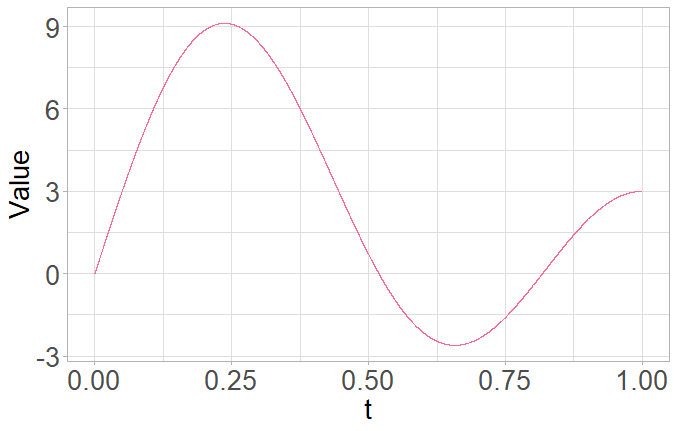
\includegraphics[width=\textwidth]{../Graphics/smooth_function.png}
  				\caption{$f_1(t)$, smooth function}
  				\label{fig:test1}
			\end{minipage}%
			\begin{minipage}{.5\textwidth}
	  			\centering
  				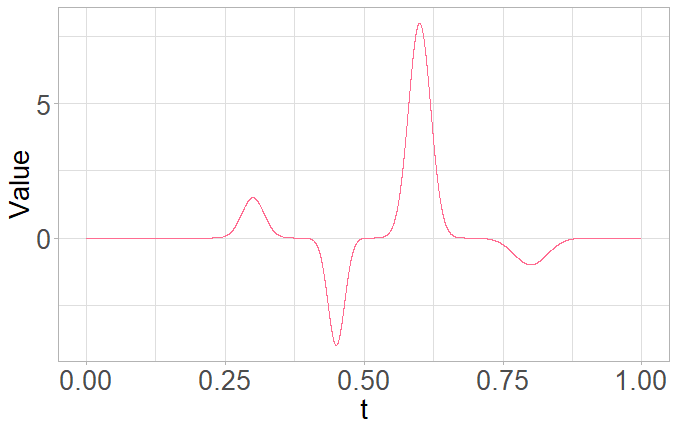
\includegraphics[width=\textwidth]{../Graphics/bumpy_function.png}
  				\caption{$f_2(t)$, bumpy function}
  				\label{fig:test2}
			\end{minipage}
		\end{figure}
		
		 Two different error-terms $\epsilon$ were created by first generating an $i.i.d.$ standard normal error term and then multiplying it by two error variations $\sigma_e $. The error variations represent different signal-to-noise ratios to test the methods both with a low and a high amount of noise. They are created such that the squared multiple correlation coefficient $R^2 = var(Xf) / (var(Xf) + \sigma^2_{e})$ is equal to 0.9 and 0.6. The two error-terms are then used to generate two sets of responses for $f \in \{f_1(t), f_2(t)\}$
		
		\begin{equation}
			\begin{split}
				Y_{1,f} & = \langle NIR, f\rangle + Z  \biggl\lbrack\frac{var(\langle NIR, f\rangle)}{0.9} - var(\langle NIR, f\rangle)\biggr\rbrack \\
				Y_{2,f} & = \langle NIR, f\rangle + Z  \biggl\lbrack\frac{var(\langle NIR, f\rangle)}{0.6} - var(\langle NIR, f\rangle)\biggr\rbrack
			\end{split}
		\end{equation}
		
		where $Z \sim \mathcal{N}(0,1)$. In total, we created four combinations for the simulations, using the two true coefficient functions and the two sets of responses. These four combinations are then used with a different number of monomial basis functions $ \in \{1,2, \dots, 6\}$, cubic bspline basis-function $\{5,6,...,18\}$ and fourier functions $\{1,3,...,25\}$ to predict the generated responses using the basis expansion approach and the FPCR approach. For the evaluation, we used the prediction RMSE calculated by 10 fold cross-validation.
		 To obtain valid out of sample properties for the FPCR, within each of the ten 10 fold cross-validation splits, we first calculate the Functional Principal Components of the trainig-set $\mathcal{T}$ for each curve. These scores are then used to estimate the scores of the holdout set $\mathcal{H}$, $\hat{\xi}_{i}^{m, \mathcal{H}}$  by the equation:
		 
	\begin{equation}
		\begin{split}
			\hat{\xi}_{i}^{m, \mathcal{H}} &=  \int_{0}^{1} {\color{red} \left(X_{i}^{\mathcal{H}}(s) - \hat{\mu}^{\mathcal{T}}(s)\right)} {\color{blue}\hat{\nu}^{m, \mathcal{T}} }\mathrm{d}s) 
						    = \int_{0}^{1} {\color{red}\left(\sum_{j \in \mathcal{I}} a_{i,j}^{\mathcal{H}} \phi_j(s)\right)} {\color{blue}\left(\sum_{k \in \mathcal{L}} b_{k}^{m, \mathcal{T}} \psi_{k}(s)\right)} \mathrm{d}s \\
			 &= \sum_{j \in \mathcal{I}} \left[ a_{i,j}^{\mathcal{H}}\sum_{k \in \mathcal{L}}  b_{k}^{m, \mathcal{T}} \int_{0}^{1} \phi_j(s) \psi_{k}(s)\mathrm{d}s\right]
		\end{split}
	\end{equation}
	\vspace{	0.2cm}
	
	
		 The simulation was done with R (version...). In total, 5000 repetitions were done for each set of simulations. 
		
	
	\subsection{Results}	
	
	\subsubsection{Basis Expansion Regression}
	The following results origin from the \hyperref[basis_exp_transf]{\textbf{Estimation using Basis-Representation}}, in which we transform the observed functions to perform regression of a scalar on a countable sequence of regressors, which is then tractable with typical multivariate regression theory. 
	
	\paragraph{Monomial Basis}
	Due to the high collinearity of these basis, simulations were conducted up until the sixth monomial basis, excluding the first one since this just represents a constant. For reasons outlined in {\color{green} Link chapter}, they are suited for the smooth function $f_1$ and show a better performance than bsplines for this coefficient function, but show the weakest performance for the coefficient function $f_2$. For $f_1$, the simulation selects 5(3) and for $f_2$ 5(5) monomial basis functions for the high(low) signal-to-noise ratios. This weakness is especially pronounced in the setup $f_2,Y_1$; for the high noise setup, $f_2, Y_2$ this weakness is still visible, but less strongly pronounced.
	
	\paragraph{Bspline Basis}
	Simulations with bspline basis functions were possible from 5 to 18, since from 18 onwards the simulations were running into problems concerning {\color{green} what happend here exactly?}
The smooth function $f_1$ requires only 5(4) Bspline basis functions, for the high(low)-signal-to-noise ratio to obtain the best fit for the bspline basis, which performs the worst for $f_1$. For $f_2$, 11(6) bspline basis functions are needed for the high(low) signal-to-noise ratios. For $f_2$, the bspline basis functions outperform the monomial basis, but come second to the fourier basis.
	
	\paragraph{Fourier Basis}
	For $f_1$, the simulation chooses a smaller number of fourier basis functions, 5(3) and a higher number for the bumpy function $f_2$, 9(7) for the setup with the high(low) signal-to-noise ratio. With the low signal-to-noise ratio, the simulation chooses a smaller number to account for the higher noise in the response variable. The fourier basis functions performs the best in each setup for the basis expansion regression. When recalling $f_1$ and $f_2$, both, but especially $f_1$ shows similar curvature order across the domain which contributes to the strong performance of this basis.
	\\
	
	
	For all specifications, the effect of the Bias-Variance tradeoff can be observed:: The function $f_1$ is rather smooth and not much bias is introduced here when choosing a small number of basis functions since $f_1$ lacks pronounced peculiarities. For $f_2$, higher number of basis functions are needed, resulting from the inherent peculiarities of $f_2$: We can choose a higher number of basis functions since the amount of bias is deceasing much faster in the number of basis functions than the variance is increasing, compared to $f_1$. 
	
	
	
	\subsubsection{Functional Principal Component Regression}
	The model which is used for the FPCR is described in \hyperref[fpc_exp_transf]{\textbf{Estimation using Functional Principal Components}}, in which we transform the observed functions to perform regression of a scalar on a countable sequence of regressors, which is then tractable with typical multivariate regression theory. 

	
	\paragraph{Monomial Basis}
	\paragraph{Bspline Basis}
	\paragraph{Fourier Basis}
	
	\subsubsection{Interpretation and Relevance for Application}

	\subsection{Literature}
	\begin{itemize}
		\item \cite{shonkwiler_explorations_2009}
		\item R-packages: fda, refund, mgcv
	\end{itemize}
	
	\newpage
	\section{Application}
		The application uses the insights from the previous sections to predict the octane ratings of the introduced gasoline dataset. Following the results from the simulation study,... 
		\begin{itemize}
			\item {\color{green} incorporate results of simulation study: number of basis, components, etc...}
			\item point out difficulties estimating sderror
			\item describe setup and results
\end{itemize}
	
	\subsection{Literature}
	\begin{itemize}
		\item \cite{carey_life_2002}
	\end{itemize}

	\section{Outlook}
	
	\subsection{Literature}
	\begin{itemize}
		\item \cite{James.2009} (shape-restrictions)
	\end{itemize}
	
	\newpage
	\section{Appendix}
	
	\subsection{Near-infrared (NIR) Spectroscopy}
	NIR- spectroscopy is a spectroscopic method that uses the near-infrared region of the electromagnetic spectrum (From 780 nm to 2500 nm). It therefore measures the absorption and interaction of this spectrum of radiation with the sample. NIR-spectroscopy is not only faster and cheaper than the standard test procedure – another big advantage is that it does not need a reagent and thus does not destroy the sample. It is used for analysis in different sectors and fields, like the agrochemical industry but also in healthcare. Its non-invasive nature makes it also to an asset for medical applications like the monitoring of diabetes in which NIR-spectroscopy is able to detect the worsening of the blood glucose metabolic dysfunction (cf . \cite{FR_li_et_al_2020}). In the context of this paper, the gasoline dataset which is used for the simulation and the application is constructed using NIR spectroscopy. According to \cite{Bohacs_Ovadi_Salgo1998} NIR-spectroscopy is a feasible method for the analysis of gasoline since most of the absorption that is observed within the described interval of wavelengths is due to overtones and interactions of the radiation with chemical combinations (eg.: carbon–hydrogen, carbon–carbon, carbon–oxygen, carbonyl associated groups, aromatic stretching, and deformation vibration of the hydrocarbon molecules). While this paper focuses on the prediction of the octane number of gasoline, other research focuses  on different properties of gasoline such as the olefin, naphtaenic and aromatic content (Parisi et al. 1990, as cited in \cite{Bohacs_Ovadi_Salgo1998}) or the distillation characktersitics (Pauls 1985, as cited in \cite{Bohacs_Ovadi_Salgo1998})

	
	\subsection{Basis Plots}
	
	\begin{figure}[H]\label{fourier_basis}
		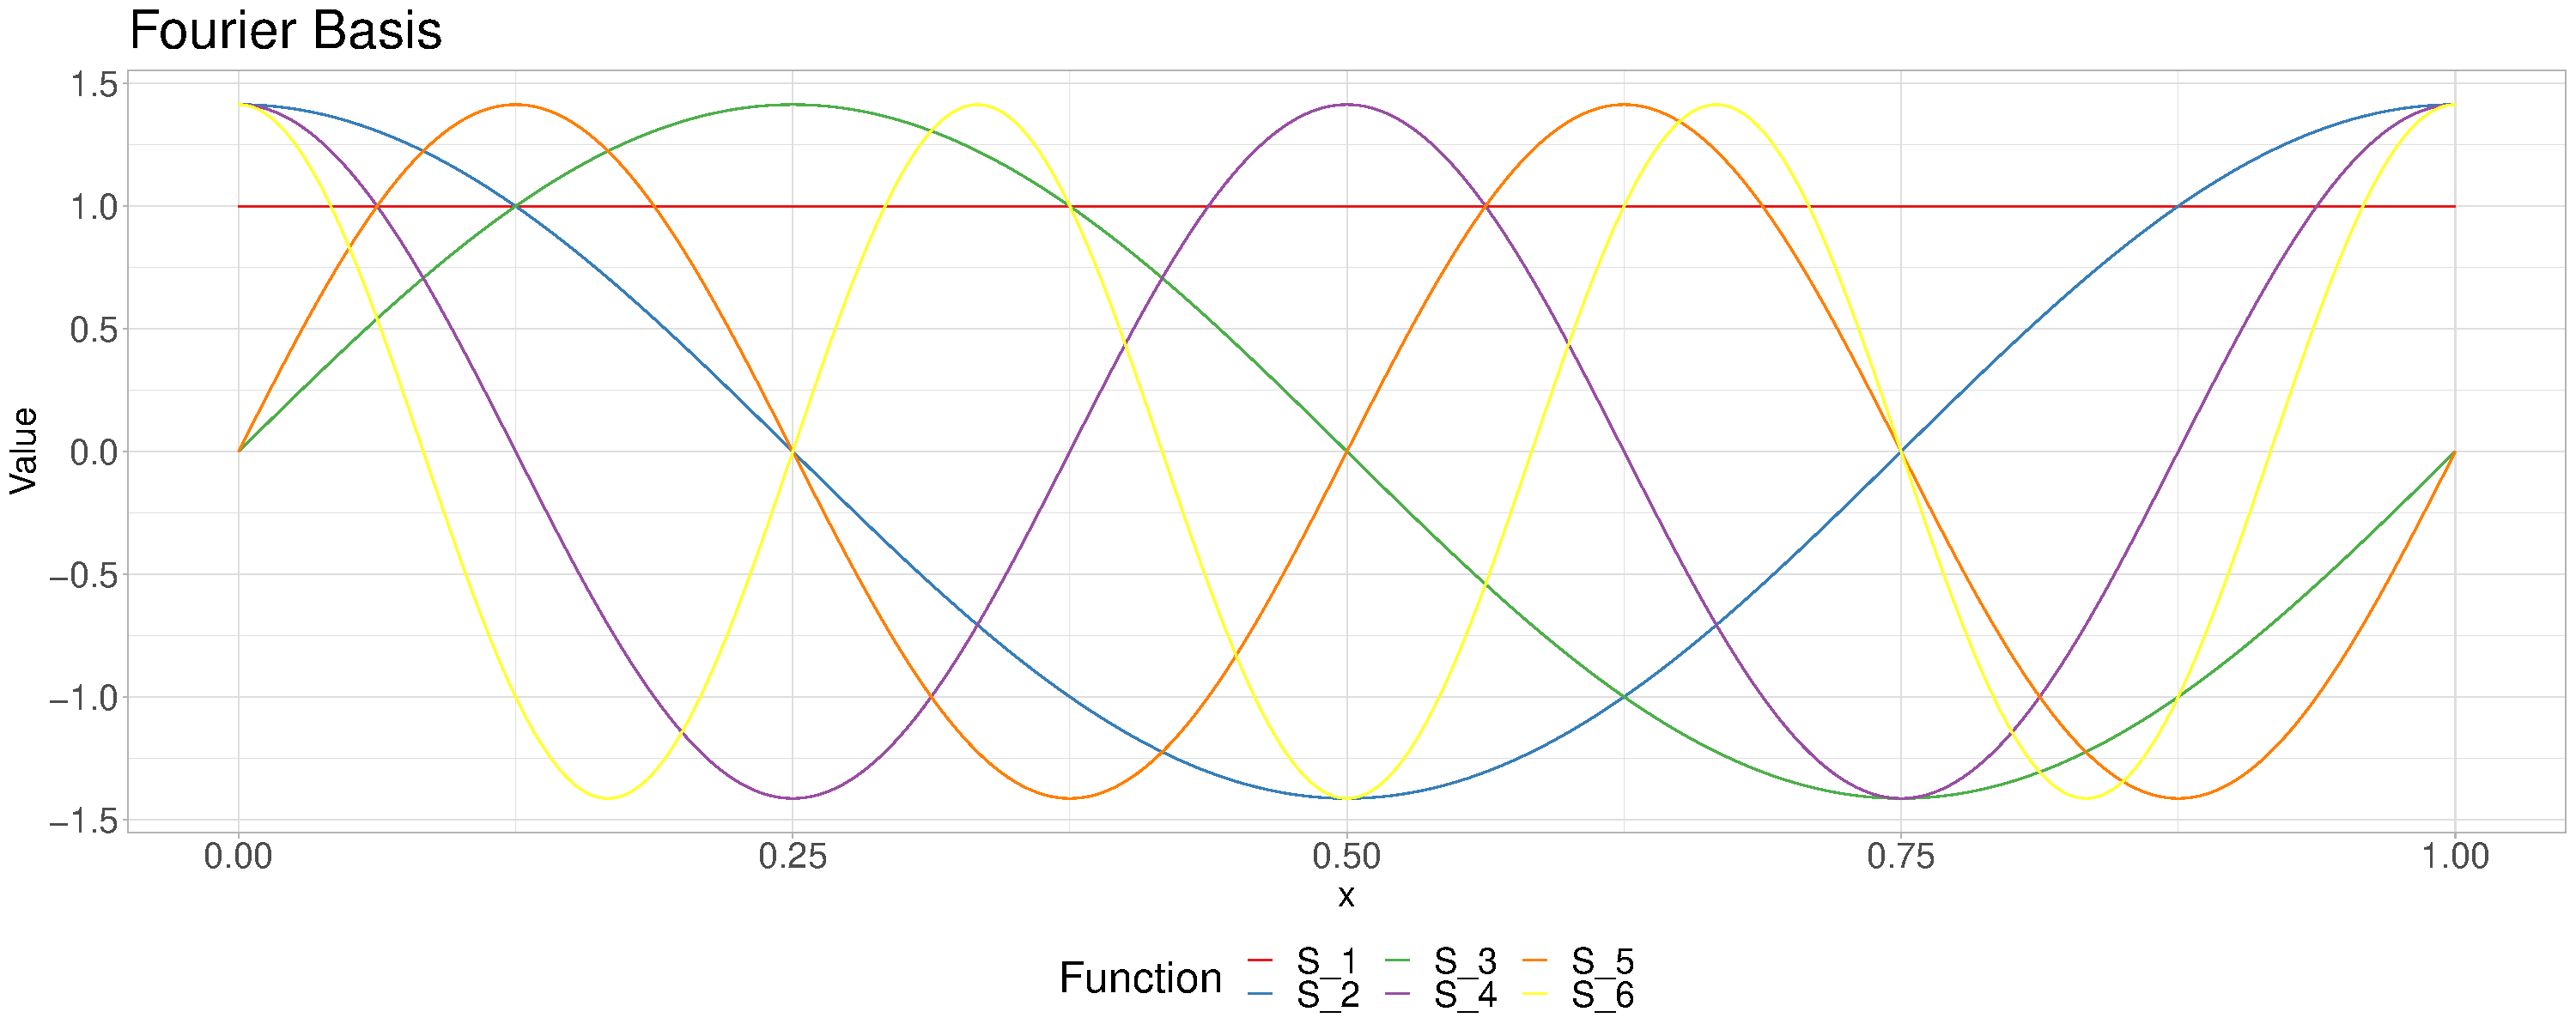
\includegraphics[width = \textwidth]{../Graphics/Fourier_Basis.pdf}
		\caption{Fourier basis functions for $i = 1,\dots,7$}
	\end{figure}
	
	\begin{figure}[H]\label{bspline_basis}
		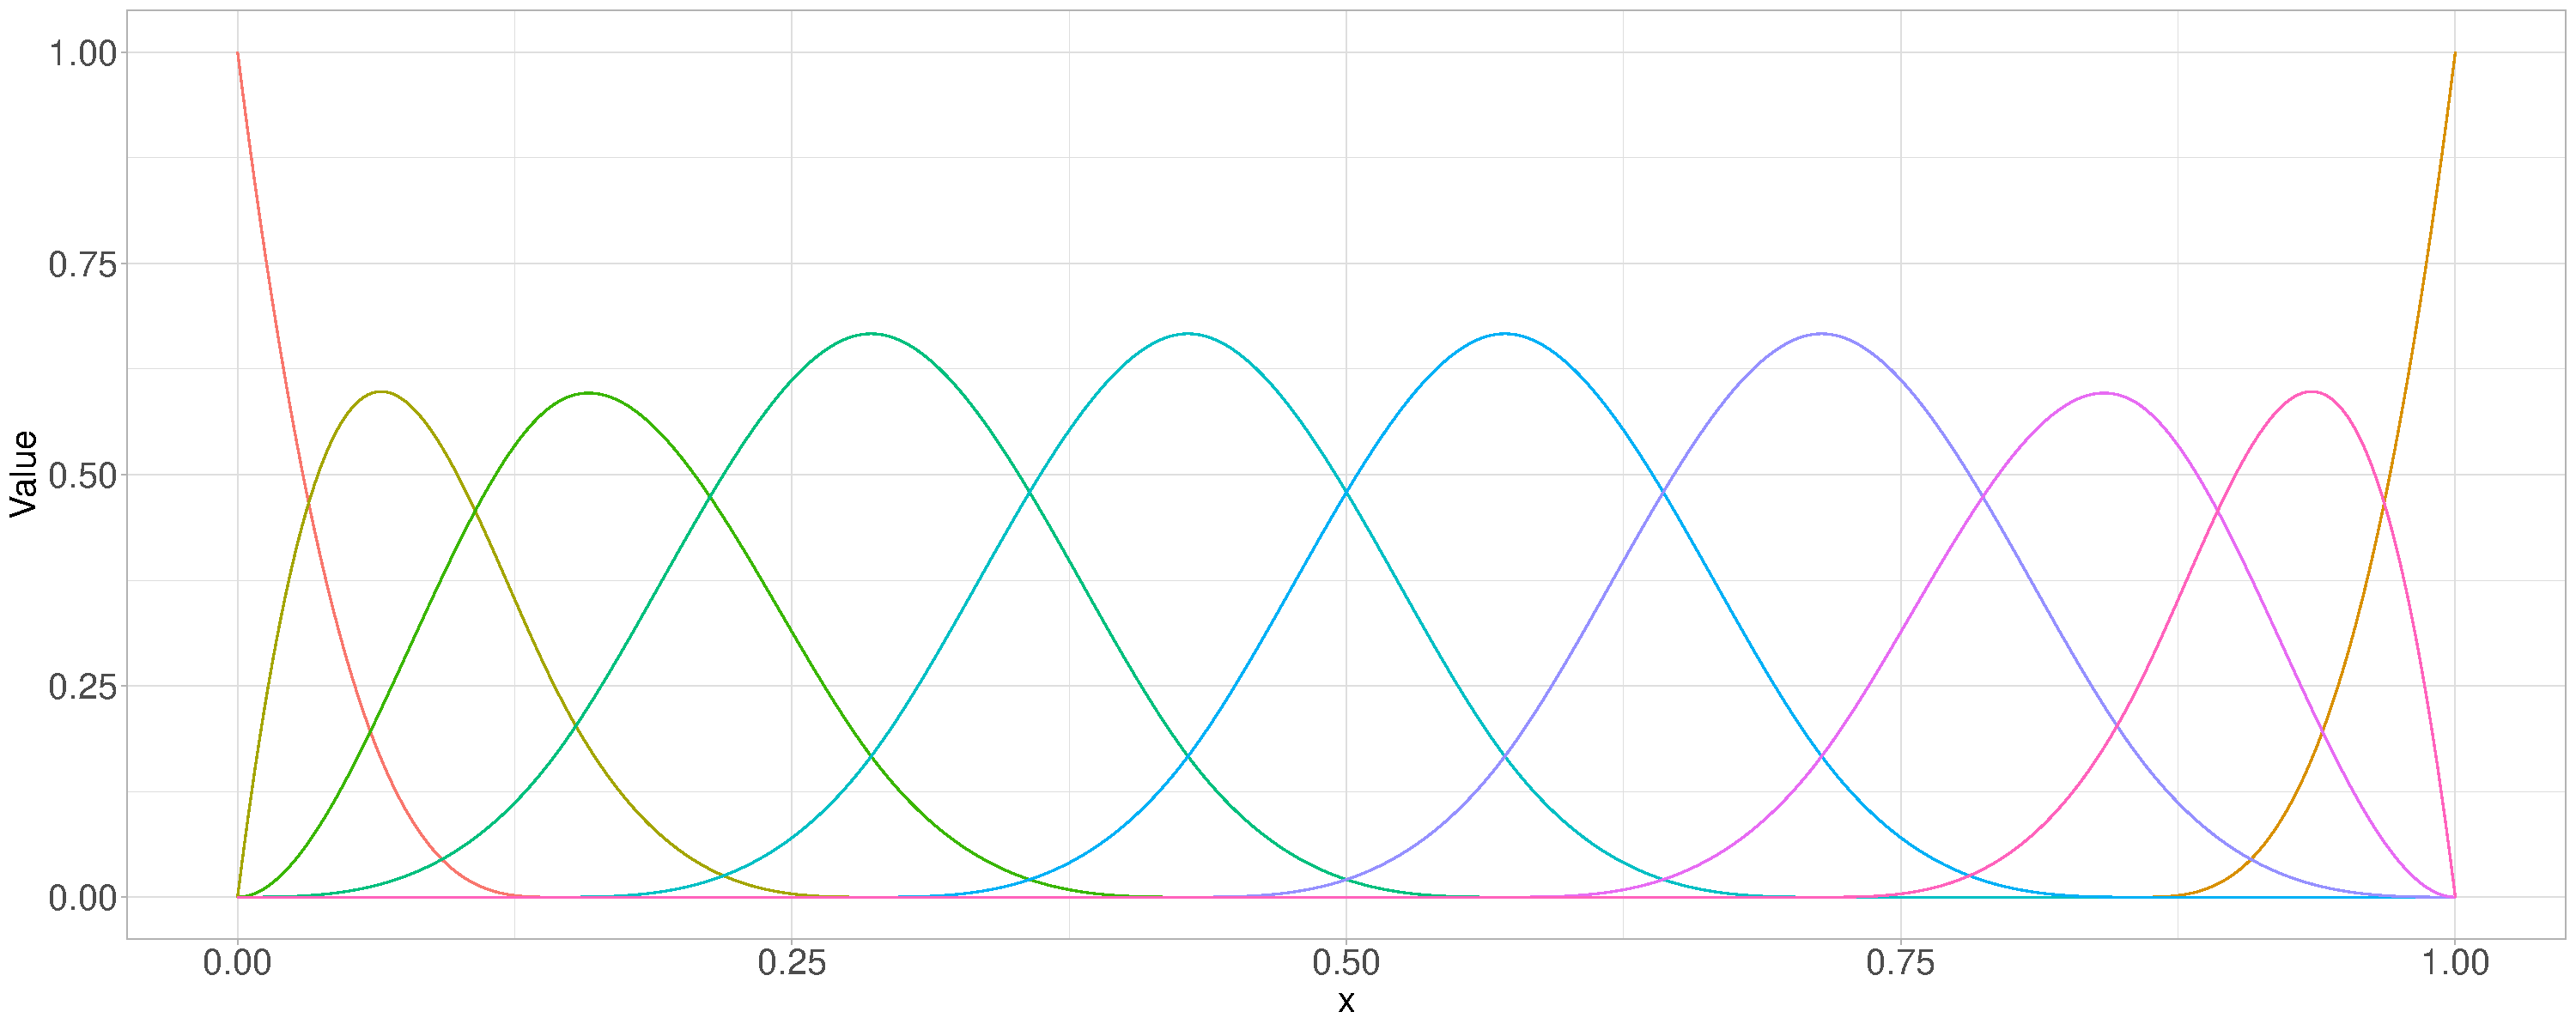
\includegraphics[width = \textwidth]{../Graphics/Bspline_Basis.pdf}
		\caption{B-spline basis functions of order 4 for 8 equidistant knots on $[0,1]$}
	\end{figure}

	\begin{figure}[H]\label{monomial_basis}
		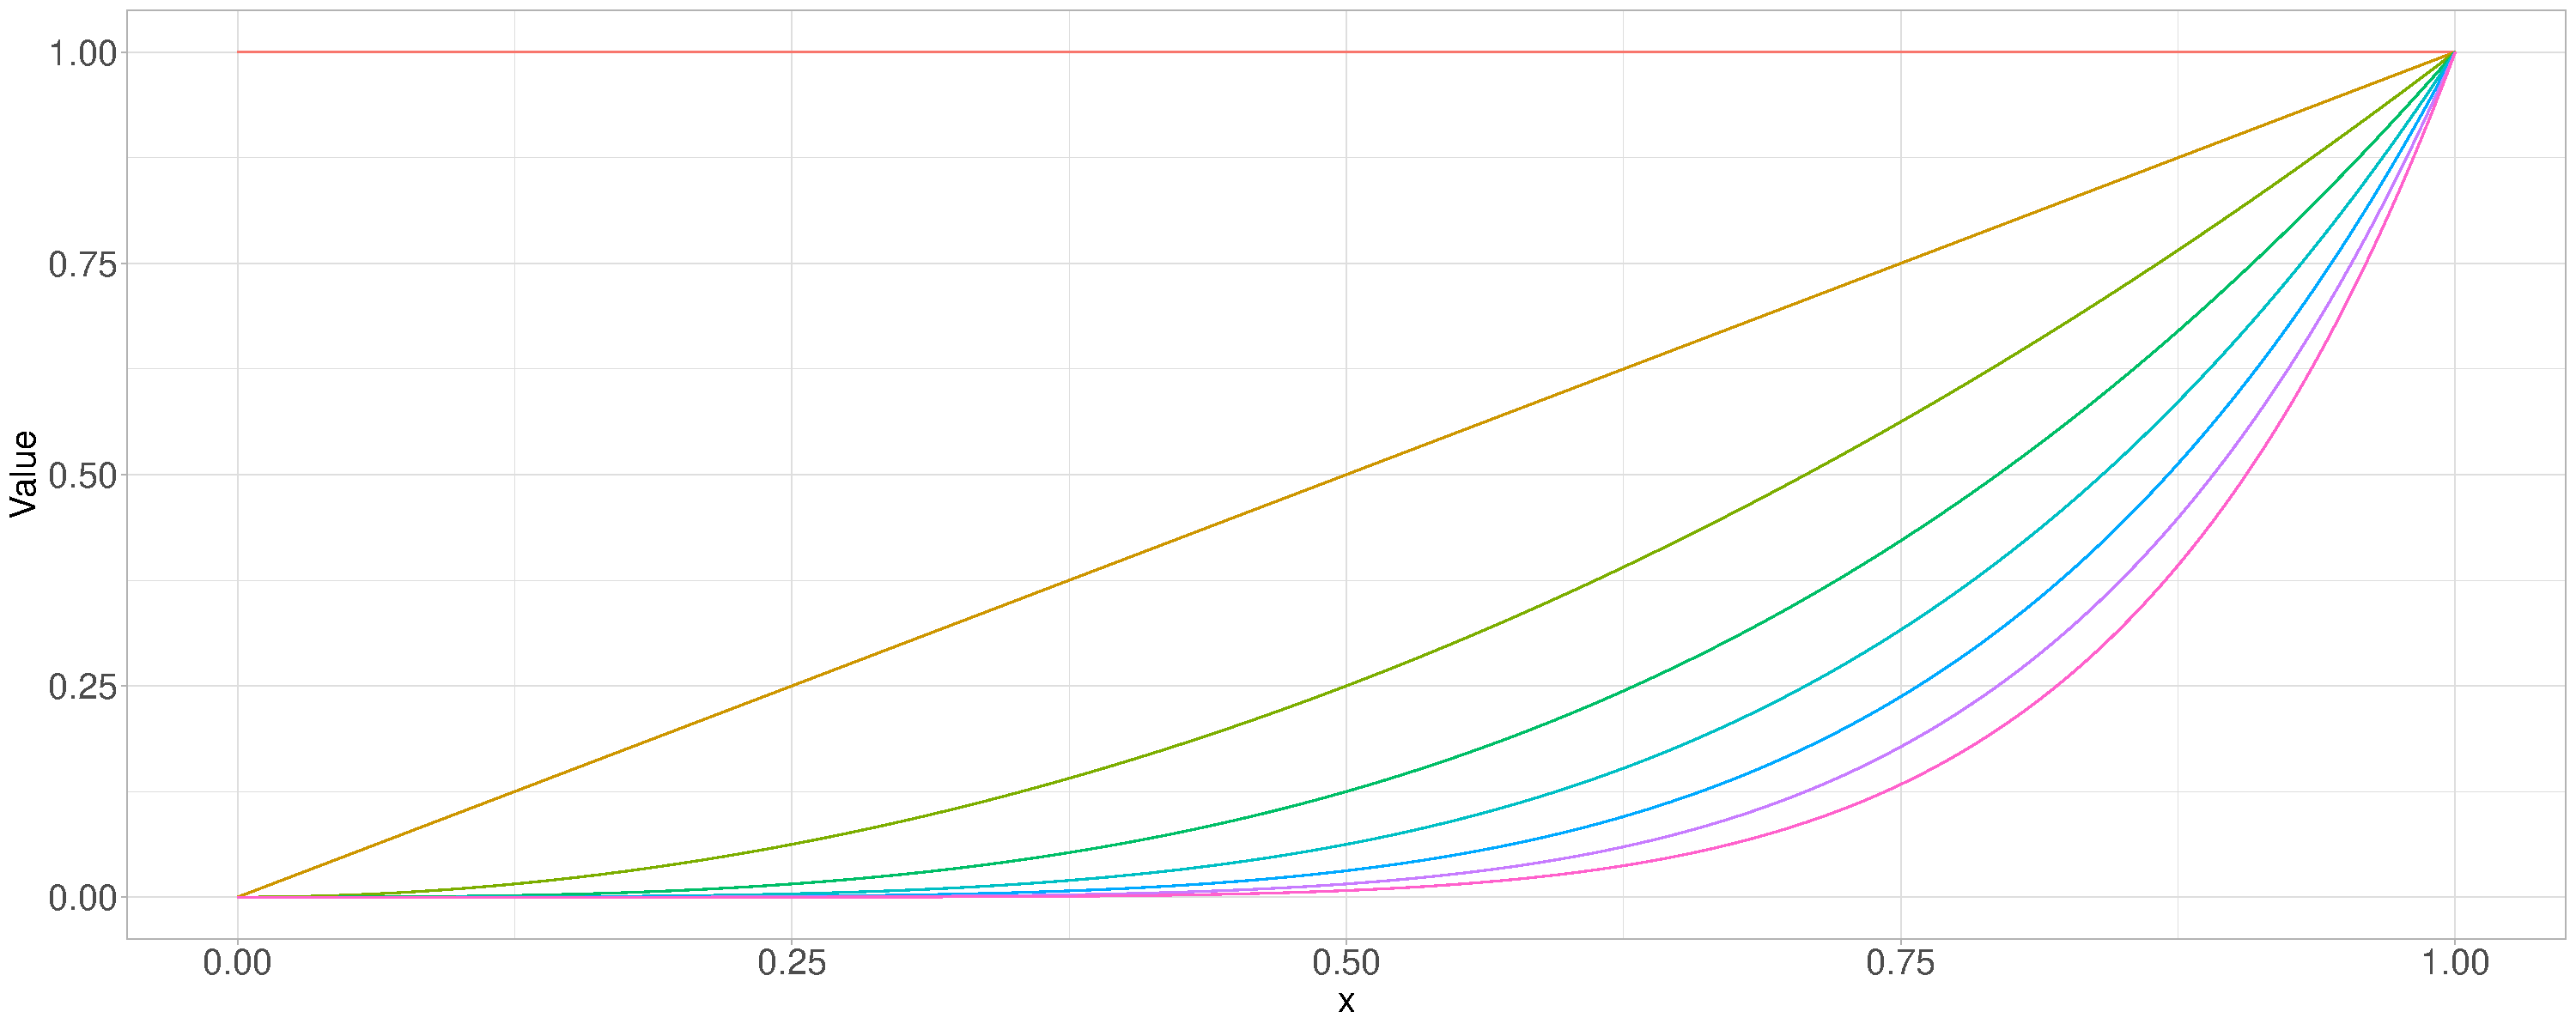
\includegraphics[width = \textwidth]{../Graphics/Monomial_Basis.pdf}
		\caption{Monomial basis functions of degree 0 to 7}
	\end{figure}

\newpage
	\subsection{Simulation Study Results}
	

	\begin{table}[htb]
			\centering
			\caption{Monomial Basis Expansion Regression}
				\begin{tabular}{lllllll}
					\cline{1-5}
					 \boldmath{$f_1, Y_1$}                 & \boldmath{$f_1, Y_2$}                  & \boldmath{$f_2, Y_1$}                    & \boldmath{$f_2, Y_2$}               & \textbf{n\_basis} &  \\ \cline{1-5}
7.177234352026647                        & 131.92716520680838                        & 0.8936725847175324                         & 2.5839516380614462                        & 2       &  \\
4.170391190343292                        & {\color[HTML]{FE0000} 129.64258934345224} & 0.8122408608804015                         & 2.511772278865247                         & 3       &  \\
3.912749103345826                        & 130.1170783435205                         & 0.3807927171910713                         & 2.090474762002978                         & 4       &  \\
{\color[HTML]{FE0000} 3.638501968909747} & 130.59817144950233                        & {\color[HTML]{FE0000} 0.09216751463887264} & {\color[HTML]{FE0000} 1.8134256416939782} & 5       &  \\
6.016442343989896                        & 201.15534584991525                        & 0.7620805051836907                         & 3.3937342332820926                        & 6       & 
\end{tabular}
\end{table}

\vspace{2cm}


	\begin{table}[htb]
			\centering
			\caption{BSpline Basis Expansion Regression}
				\begin{tabular}{lllllll}
					\cline{1-5}
					 \boldmath{$f_1, Y_1$}                 & \boldmath{$f_1, Y_2$}                  & \boldmath{$f_2, Y_1$}                    & \boldmath{$f_2, Y_2$}               & \textbf{n\_basis} &  \\ \cline{1-5}
3.9127490963955247                        & {\color[HTML]{FE0000} 130.1170783090359} & 0.3807927168700936                          & 2.090474761101881                         & 4       &  \\
{\color[HTML]{FE0000} 3.6430480624640396} & 130.61094959896604                       & 0.09511820431115069                         & 1.8164314387816713                        & 5       &  \\
3.6542611008674575                        & 131.35354539843397                       & 0.07775281510299467                         & {\color[HTML]{FE0000} 1.8091346529425483} & 6       &  \\
3.6770545937377634                        & 132.14205183557064                       & 0.07518488287219192                         & 1.8168036577708813                        & 7       &  \\
3.710740869697218                         & 133.3653658811635                        & 0.05810108378740701                         & 1.8164984632128844                        & 8       &  \\
3.7192146351418724                        & 133.6814928169343                        & 0.05640282340664383                         & 1.8193083539013821                        & 9       &  \\
3.742010447810594                         & 134.5121710907784                        & 0.0521785231194299                          & 1.8257576297312081                        & 10      &  \\
3.7643964092462974                        & 135.29727347111702                       & {\color[HTML]{FE0000} 0.051902252769905684} & 1.8360966075573522                        & 11      &  \\
3.80109308638683                          & 136.5758146586355                        & 0.052040315671138586                        & 1.8531479959118535                        & 12      &  \\
3.834360204971099                         & 137.78406681481994                       & 0.052706573106132304                        & 1.869969847032031                         & 13      &  \\
3.862166917165765                         & 138.73431326927349                       & 0.053068654178390816                        & 1.8826933364948355                        & 14      &  \\
3.8685638723557956                        & 138.97427074660192                       & 0.0525955164519272                          & 1.8848221385552892                        & 15      &  \\
3.88505750612787                          & 139.57418873526626                       & 0.05283448721173191                         & 1.8933474257957223                        & 16      &  \\
3.912671952971778                         & 140.51490301138338                       & 0.053220205231306356                        & 1.9061942087104604                        & 17      &  \\
3.948125713522542                         & 141.80885020010606                       & 0.053584434348457485                        & 1.9231184762987383                        & 18      & 
\end{tabular}
\end{table}


\vspace{2cm}


	\begin{table}[htb]
			\centering
			\caption{Fourier Basis Expansion Regression}
				\begin{tabular}{lllllll}
					\cline{1-5}
					 \boldmath{$f_1, Y_1$}                 & \boldmath{$f_1, Y_2$}                  & \boldmath{$f_2, Y_1$}                    & \boldmath{$f_2, Y_2$}               & \textbf{n\_basis} &  \\ \cline{1-5}
3.6975216821108177                        & {\color[HTML]{FE0000} 129.19133735032568} & 0.6952364931614831                         & 2.394399533437222                         & 3       \\
{\color[HTML]{FE0000} 3.6347035142043147} & 130.59281554182246                        & 0.07418129892625985                        & 1.795816800944426                         & 5       \\
3.6762259845089287                        & 132.0824820138016                         & 0.05147130962678385                        & {\color[HTML]{FE0000} 1.7934269021325526} & 7       \\
3.718852537544315                         & 133.67575428625497                        & {\color[HTML]{FE0000} 0.05104970622270979} & 1.812908100982769                         & 9       \\
3.764506721475903                         & 135.26218648523314                        & 0.05146451789575423                        & 1.8346302450265894                        & 11      \\
3.810949927900835                         & 136.90281800923086                        & 0.05197380387819929                        & 1.8572425102431276                        & 13      \\
3.8567441840723165                        & 138.57257529224665                        & 0.05252120988973837                        & 1.8802107534919845                        & 15      \\
3.9061852571557436                        & 140.29178124765565                        & 0.05304327165297495                        & 1.9028253007284568                        & 17      \\
3.9551703628111876                        & 142.057266882177                          & 0.053647142499864804                       & 1.9271845824346567                        & 19     
\end{tabular}
\end{table}






\subsection{Wiener Process}\label{Wiener}
A Wiener process $W_t$ is a real-valued continuous-time stochastic process {\color{red} ... This is wikipedia, look for right citation!}
It is characterized by the following properties.

\begin{multicols}{2}
	\begin{enumerate}
		\item $W_0 = 0$
		\item $\forall t > 0 W_{t+u} - W_t \perp\!\!\!\perp W_s \forall s \leq t$
		\item $W_{t+u} - W_t \sim \mathcal{N}(0,u)$
		\item $W_t$ is continuous in $t$
	\end{enumerate}
\end{multicols}

\begin{figure}[H]\label{Wiener_plot}
	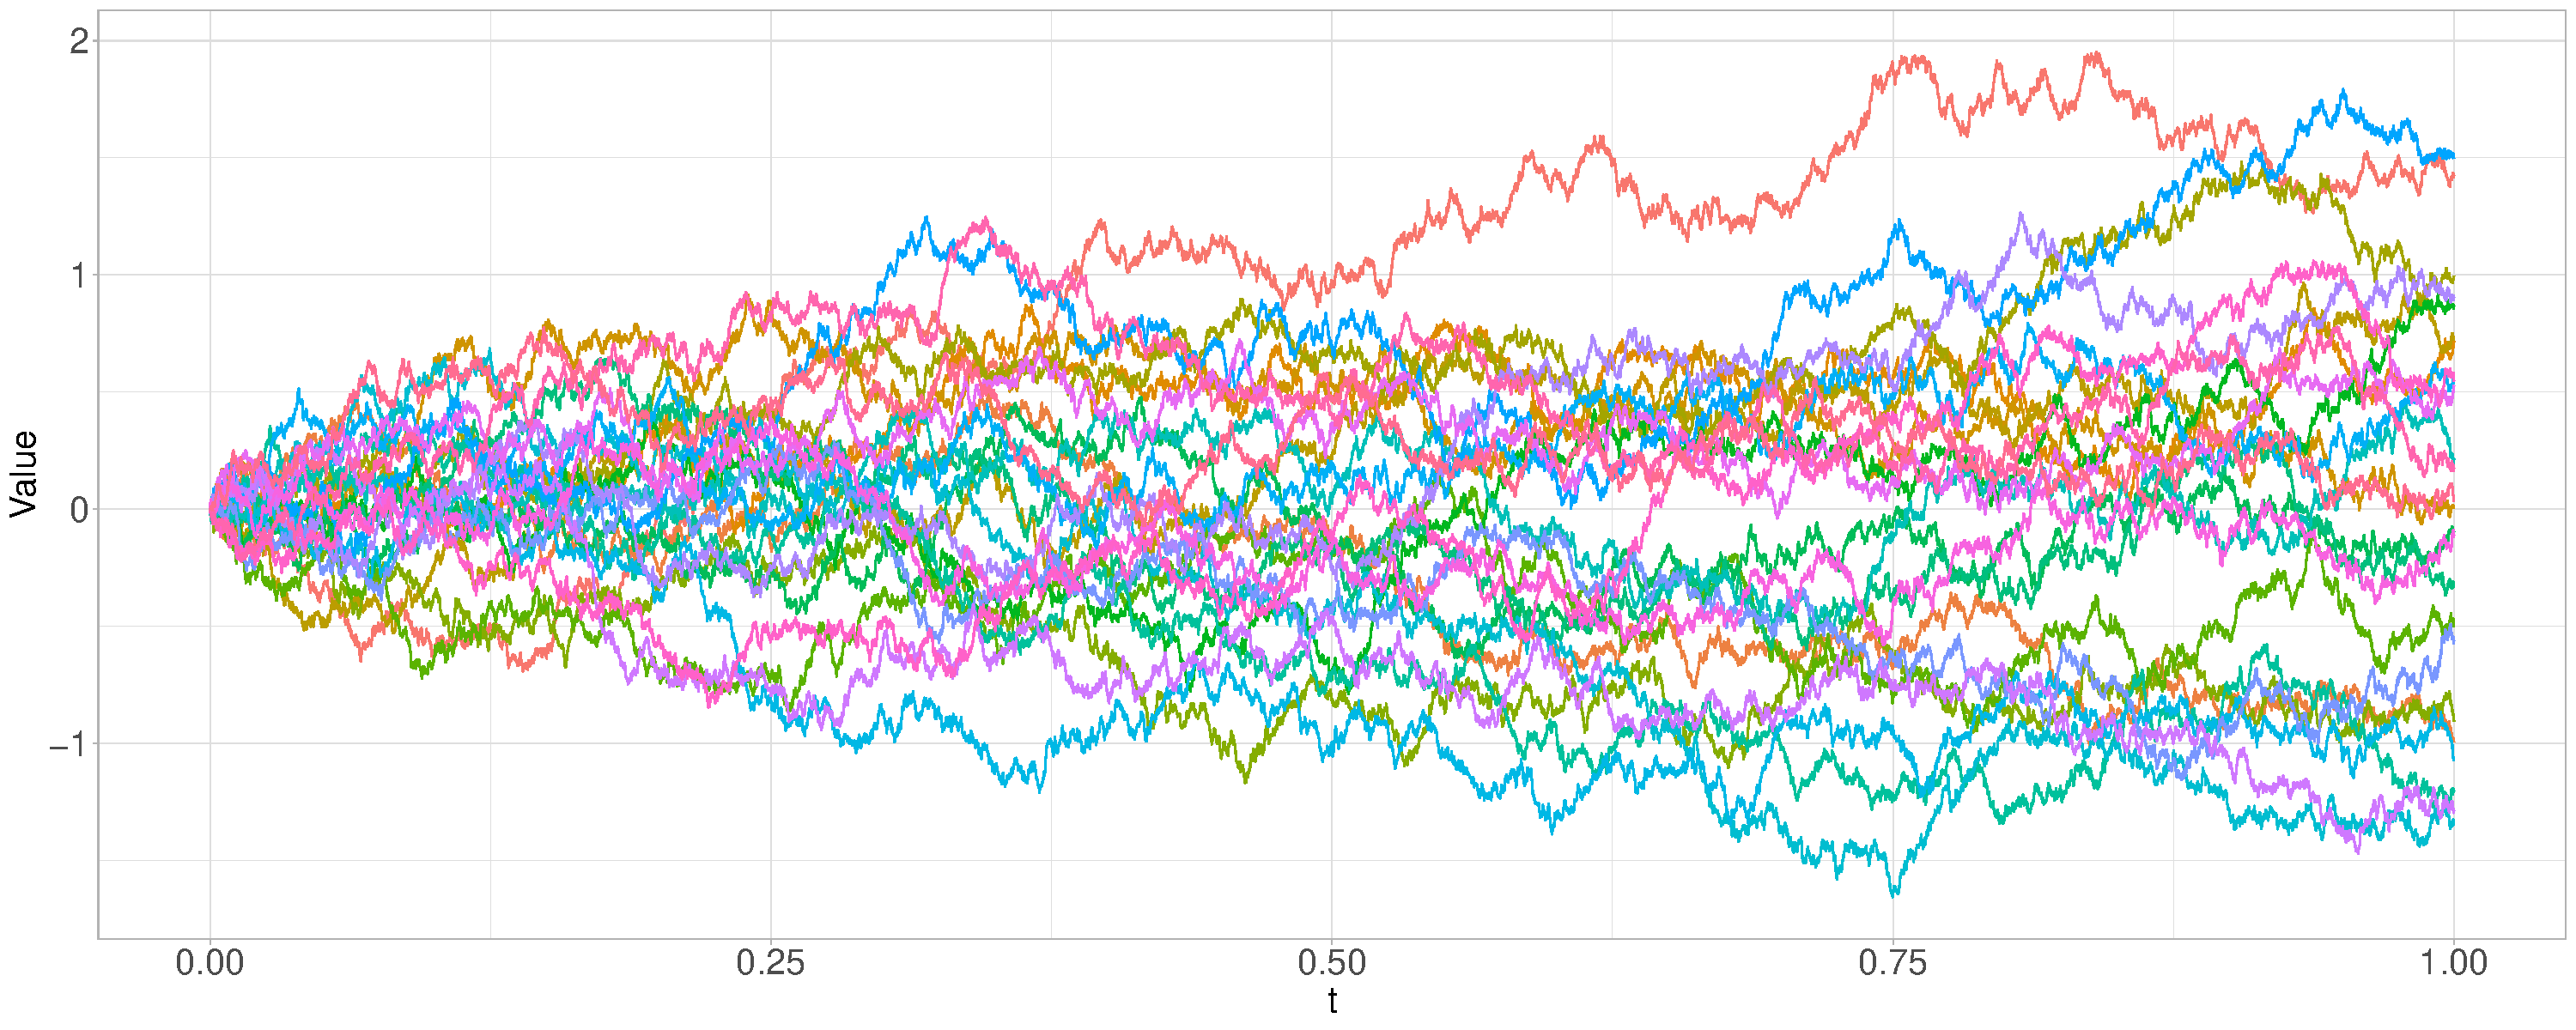
\includegraphics[width = \textwidth]{../Graphics/Wiener_plot.pdf}
	\caption{25 i.i.d. realizations of a Wiener Process on $[0,1]$}
\end{figure}

	\section{Proofs}
	\subsection{Lemma} \label{Proof1}
	{\color{orange} We might put the below theorems for KL. The deterministic basis expansions are pretty clear about why we can use the truncation version by itself. In contrast, I feel like that for the case of KL it does not. And in the centered case?} 
	The coefficients $\xi_{j}$ satisfy the following:
	\begin{enumerate}
		\item $\mathbb{E}[\xi_{j}] = 0$
		\item $\mathbb{E}[\xi_{j} \xi_{k}] = \lambda_{j}$, if $j = k$, otherwise 0
		\item Var[$\xi_{j}$] = $\lambda_{j}$
	\end{enumerate}
	
	\begin{proof}
		To obtain the first result, we can show that
		\begin{equation}
			\begin{split}
				\mathbb{E}[\xi_{j}] = & \mathbb{E} \biggl\lbrack \int_{0}^{1} F(t) \nu_{j}(t)dt \biggr\rbrack\\
				= & \int_{\Omega} \int_{0}^{1} F(t) \nu_{j}(t) dt dP(\omega)\\
				= & \int_{0}^{1} \int_{\Omega} F(t) \nu_{j}(t) dP(\omega) dt \quad \text{(Fubini)}\\
				= & \int_{0}^{1} \mathbb{E}[F(t)] \nu_{j}(t) dt\\
				= & \mu(t) \int_{0}^{1} \nu_{j}(t)\\
				= & \mu(t) \langle \nu_{j}(t), 1 \rangle = 0
			\end{split}
		\end{equation}
		where the constant function is always an eigenfunction of the operater $K$. It leads the inner product to 0 due to orthonormality of eigenfunctions. {\color{red} Another way to prove or use centered mean}
		For the case of centered process
		\begin{equation}\label{Lemma1}
			\begin{split}
				\mathbb{E}[\xi_{j}] = & \mathbb{E} \biggl\lbrack \int_{0}^{1} F(t) \nu_{j}(t)dt\biggr\rbrack\\
				= & \int_{\Omega} \int_{0}^{1} F(t) \nu_{j}(t) dt dP(\omega)\\
				= & \int_{0}^{1} \int_{\Omega} F(t) \nu_{j}(t) dP(\omega) dt \quad \text{(Fubini)}\\
				= & \int_{0}^{1} \int_{\Omega} F(t) dP(\omega) \nu_{j}(t) dt\\
				= & \int_{0}^{1} \mathbb{E}[F(t)] \nu_{j}(t) dt = 0
			\end{split}
		\end{equation}
		where $\mathbb{E}[F(t)]$ is 0 since $F(t)$ is a centered process.
		The second claim is proved as:
		\begin{equation}\label{Lemma2}
			\begin{split}
				\mathbb{E} [\xi_{j} \xi_{k}] = & \mathbb{E}  \biggl\lbrack \int_{0}^{1} F(s) \nu_{j}(s)ds \int_{0}^{1} F(t) \nu_{k}(t)dt  \biggr\rbrack\\
				= & \mathbb{E} \biggl\lbrack {\int_{0}^{1} \int_{0}^{1} F(s) \nu_{j}(s) F(t) \nu_{k}(t) ds dt} \biggr\rbrack \quad \text{(Fubini)}\\
				= & \int_{0}^{1} \int_{0}^{1} {\color{red}\mathbb{E}[{F(s)F(t)}]} \nu_{j}(s) \nu_{k}(t) ds dt\\
				= & \int_{0}^{1} {\color{red}\left(\int_{0}^{1}c(s,t)\nu_{j}(s)ds \right)} \nu_{k}(t) dt \\
				= & \int_{0}^{1}{\color{red}[K\nu_{j}](t)}\nu_{k}(t)dt\\
				= & \langle K \nu_{j}, \nu_{k} \rangle\\
				= & \langle \lambda_{j} \nu_{j}, \nu_{k} \rangle = \lambda_{j} \quad \text{if $j = k$, otherwise 0}
			\end{split}
		\end{equation}
		where the result is produced from orthonormaility of the eigenfunctions. The last assertion is confirmed from the other two properties.
		\begin{equation}\label{Lemma3}
			Var[\xi_{i}] = \mathbb{E}\left[(\xi_{i} - \mathbb{E}[\xi_{i}])^{2}\right] = \mathbb{E}[\xi_{i}^{2}] = \lambda_{i}
		\end{equation}
	\end{proof}
	
	
	\subsection{Karhunen-Lo\'{e}ve expansion} \label{Proof2}
	Let $F : [0,1]  \rightarrow \mathbb{R}$ be a centered mean-square continuous stochastic process with $F \in \mathbb{L}^{2}[0,1]$. Then there exists a basis ${\xi_{i}}$ of $\mathbb{L}^2[0,1]$ such that for all $t \in [0,1]$,
	\begin{equation}
		F(t) = \sum_{j=1}^{\infty} \xi_{j} \nu_{j}(t),
	\end{equation}
	where coefficients $\xi_{j}$ are given by $\xi_{j}(\omega) = \int_{0}^{1} F(t)(\omega) \nu_{j}(t)dt$ and satisfy the following conditions.
	\begin{enumerate}
		\item $\mathbb{E}[\xi_{j}] = 0$
		\item $\mathbb{E}[\xi_{j} \xi_{k}] = \lambda_{j}$, if $j = k$, otherwise 0
		\item Var[$\xi_{j}$] = $\lambda_{j}$
	\end{enumerate}
	
	\begin{proof}
		We know that $K$ has a complete set of eigenvectors ${\nu_{j}}$ in $\mathbb{L}^{2}[0,1]$ and non-negative eigenvalues $\lambda_{j}$. With the fact that $\xi_{j}(\omega) = \int_{0}^{1} F(\omega)(t) \nu_{j}(t)dt$ satisfy the three conclusions by Lemma. We prove it by considering
		\begin{equation}
			\epsilon_{n}(t) := \mathbb{E} \left[\bigg( F(t) - \sum_{j=1}^{n} \xi_{j} \nu_{j}(t)\bigg)^2 \right]
		\end{equation}
		
		Once it is shown that $\lim\limits_{n \rightarrow \infty} \epsilon_{n}(t) = 0$ uniformly in [0,1], the proof is completed.
		\begin{equation}\label{Thr1}
			\begin{split}
				\epsilon_{n}(t) = &\mathbb{E} \left[\bigg( F(t) - \sum_{j=1}^{n} \xi_{j} 	\nu_{j}(t)\bigg)^2 \right]\\
				= & \mathbb{E}[F(t)^{2}] - 2\mathbb{E}\bigg[F(t)\sum_{j=1}^{n}\xi_{j}\nu_{j}(t)\bigg] + \mathbb{E}\bigg[\sum_{j=1}^{n}\sum_{k=1}^{n}\xi_{j}\xi_{k}\nu_{j}(t)\nu_{k}(t)\bigg]
			\end{split}
		\end{equation}
		
		Now, $\mathbb{E}[F(t)^{2}] = c(t,t)$ as in (\ref{CovarianceFunction}),
		\begin{equation}\label{Thr2}
			\begin{split}
				\mathbb{E} \bigg[ F(t) \sum_{j=1}^{n} \xi_{j}\nu_{j}(t) \bigg] = & \mathbb{E} \left[ F(t) \sum_{j=1}^{n} \bigg(\int_{0}^{1} F_{s}\nu_{i}(s)ds\bigg) \xi_{j}(t) \right]\\
				= & \sum_{j=1}^{n} \bigg(\int_{0}^{1} \mathbb{E}[F(t)F(s)]\nu_{j}(s)ds\bigg)\nu_{j}\\
				= & \sum_{j=1}^{n} \bigg(\int_{0}^{1} c(t,s) \nu_{j}(s)ds\bigg)\nu_{j}\\
				= & \sum_{j=1}^{n}[K\nu_{j}](t)\nu_{j} = \sum_{j=1}^{n}\lambda_{j}\nu_{j}^{2}
			\end{split}
		\end{equation} 
		
		We derive from (\ref{Lemma2}) that
		\begin{equation}\label{Thr3}
			\begin{split}
				\mathbb{E}\bigg[\sum_{j=1}^{n} \sum_{k=1}^{n} \xi_{j} \xi_{k} \nu_{j}(t) \nu_{k}(t)\bigg] = & \sum_{j=1}^{n} \sum_{k=1}^{n} \mathbb{E}[\xi_{j} \xi_{k}] \nu_{j}(t) \nu_{k}(t)\\
				= & \sum_{j=1}^{n} \sum_{k=1}^{n} \delta_{jk} \lambda_{j} \nu_{j}(t) \nu_{k}(t) = 		\sum_{j=1}^{n} \lambda_{j} \nu_{j}(t)^{2}
			\end{split}	
		\end{equation}
		where $\delta_{jk} = 1$ if $j=k$, otherwise 0. Therefore, by (\ref{Thr1}), (\ref{Thr2}), and (\ref{Thr3}) we obtain
		\begin{equation}
			\epsilon_{n}(t) = c(t,t) - \sum_{j=1}^{n} \lambda_{j} \nu_{j}(t) \nu_{j}(t)
		\end{equation}
		
		implementing Mercer's Theorem this proof is concluded by
		\begin{equation}
			\lim\limits_{n \rightarrow \infty} \epsilon_{n}(t) = \lim\limits_{n \rightarrow \infty} \mathbb{E} \left[\bigg( F(t) - \sum_{j=1}^{n} \xi_{j} \nu_{j}(t)\bigg)^2 \right] = 0
		\end{equation}
	\end{proof}

	\newpage
	
	\section{Bibliography}
	\printbibliography[heading=none]	
	
	\newpage
	\section{Affidavit}
	
	\vspace{2cm}
	"I hereby confirm that the work presented has been performed and
	interpreted solely by myself except for where I explicitly identified the
	contrary. I assure that this work has not been presented in any other
	form for the fulfillment of any other degree or qualification. Ideas
	taken from other works in letter and in spirit are identified in every
	single case."
	
	\vspace{2cm}
	Bonn, 11.02.2021 \hrulefill \\
	\hspace*{0mm}Jonghun Baek
	
	\vspace{2cm}
	Bonn, 11.02.2021 \hrulefill \\
	\hspace*{0mm}Jakob R. Juergens
	
	\vspace{2cm}
	Bonn, 11.02.2021 \hrulefill \\
	\hspace*{0mm}Jonathan Willnow
	
	
\end{document}